\documentclass[12pt,a4paper]{report}

\usepackage{styles/dolgozat}

\usepackage{listings}
\usepackage{styles/cpp}
\usepackage{styles/python}

\usepackage{hyperref}

\begin{document}

\pagestyle{empty} %a címlapon ne legyen semmi=empty, azaz nincs fejléc és lábléc

% A Miskolci Egyetem címere
{\large
\begin{center}
\vglue 1truecm
\textbf{\huge\textsc{Szakdolgozat}}\\
\vglue 1truecm

\includegraphics[width=4.8truecm, height=4truecm]{images/me_logo.png}\\
\textbf{\textsc{Miskolci Egyetem}}
\end{center}}

\vglue 1.5truecm %függõleges helykihagyás

% A szakdolgozat címe, akár több sorban is
{\LARGE
\begin{center}
\textbf{Interaktív megjelenítő eszköz pénzügyi adatok elemzéséhez}
\end{center}}

\vspace*{2.5truecm}
% A hallgató neve, évfolyam, szak(ok), a konzulens(ek) neve
{\large
\begin{center}
\begin{tabular}{c}
\textbf{Készítette:}\\
Bencze Zsombor\\
Programtervező informatikus
\end{tabular}
\end{center}
\begin{center}
\begin{tabular}{c}
\textbf{Témavezető:}\\
Dr. Karácsony Zsolt
\end{tabular}
\end{center}}
\vfill
% Keltezés: Hely, év
{\large
\begin{center}
\textbf{\textsc{Miskolc, 2023}}
\end{center}}

\newpage


\newpage

\pagestyle{empty}

%Feladatkiiras
\begin{flushleft}
\textsc{\bfseries Miskolci Egyetem}\\
Gépészmérnöki és Informatikai Kar\\
Alkalmazott Matematikai Intézeti Tanszék\hspace*{4cm}\hfil \textbf{Szám:}
\end{flushleft}
\vskip 0.5cm
\begin{center}
\large\textsc{\bfseries Szakdolgozat Feladat}
\end{center}
\vskip 0.5cm
Bencze Zsombor (LP5J4B) Programtervező informatikus jelölt részére.\newline

\noindent\textbf{A szakdolgozat tárgyköre:} Webfejlesztés, pénzügy\newline

\noindent\textbf{A szakdolgozat címe:} Interaktív megjelenítő eszköz pénzügyi adatok elemzéséheze\newline

\noindent\textbf{A feladat részletezése:}

\medskip

\emph{A szakdolgozat célja olyan interaktív, dinamikus megjelenítési módok tervezésének, működésének és használatának a bemutatása, amelyekkel egyazon idősor különböző részei, különböző forrásból származó idősorok, az azokból származtatott értékek összehasonlíthatók, az aggregáláshoz használt paraméterek rugalmasan változtathatók.}

\medskip

\emph{A pénzügyi adatok (például tőzsdei árfolyamok) elemzéséhez elengedhetetlen, hogy a rendelkezésre álló információk a szakértők számára könnyen áttekinthető formában rendelkezésre álljanak}

\medskip

\emph{Az alkalmazásnak webes környezetben, szerver-kliens architektúrának megfelelően kell elkészülnie. Ehhez szerver oldalon Node.JS programnyelvet fogok használni. Míg a kliens weboldal megvalósításához HTML5, CSS, JavaScript programnyelveket kell használni.}

\vfill

\noindent\textbf{Témavezető:} Dr. Karácsony Zsolt (egyetemi docens) \newline

% \noindent\textbf{Konzulens(ek):} (akkor kötelezõ, ha a témavezetõ nem valamelyik matematikai tanszékrõl való; de persze lehet egyébként is)\newline

\noindent\textbf{A feladat kiadásának ideje:} 2023. február 16.\newline

%\noindent\textbf{A feladat beadásának határideje:}

\vskip 2cm

\hbox to \hsize{\hfil{\hbox to 6cm {\dotfill}\hbox to 1cm{}}}

\hbox to \hsize{\hfil\hbox to 3cm {szakfelelős}\hbox to 2cm{}}

\newpage

\vspace*{1cm}  
\begin{center}
\large\textsc{\bfseries Eredetiségi Nyilatkozat}
\end{center}
\vspace*{2cm}  

Alulírott \textbf{Bencze Zsombor}; Neptun-kód: \texttt{LP5J4B} a Miskolci Egyetem Gépészmérnöki és Informatikai Karának végzős Programtervező informatikus szakos hallgatója ezennel büntetőjogi és fegyelmi felelősségem tudatában nyilatkozom és aláírásommal igazolom, hogy \textit{ Interaktív megjelenítő eszköz pénzügyi adatok elemzéséheze}
című szakdolgozatom saját, önálló munkám; az abban hivatkozott szakirodalom
felhasználása a forráskezelés szabályai szerint történt.\\

Tudomásul veszem, hogy szakdolgozat esetén plágiumnak számít:
\begin{itemize}
\item szószerinti idézet közlése idézőjel és hivatkozás megjelölése nélkül;
\item tartalmi idézet hivatkozás megjelölése nélkül;
\item más publikált gondolatainak saját gondolatként való feltüntetése.
\end{itemize}

Alulírott kijelentem, hogy a plágium fogalmát megismertem, és tudomásul veszem, hogy
plágium esetén szakdolgozatom visszautasításra kerül.

\vspace*{3cm}

\noindent Miskolc, \hbox to 2cm{\dotfill} .év \hbox to 2cm{\dotfill} .hó \hbox to 2cm{\dotfill} .nap

\vspace*{3cm}

\hspace*{8cm}\begin{tabular}{c}
\hbox to 6cm{\dotfill}\\
Hallgató
\end{tabular}



\newpage

\noindent 1.

\begin{tabular}{cl}
&szükséges (módosítás külön lapon) \\
A szakdolgozat feladat módosítása& \\
& nem szükséges\\
&\\
\hbox to 4cm{\dotfill}&\multicolumn{1}{c}{\hbox to 5cm{\dotfill}}\\
dátum& \multicolumn{1}{c}{témavezető(k)}
\end{tabular}
\vskip1.5mm

\noindent 2. A feladat kidolgozását ellenőriztem:

\vskip1.5mm

\begin{tabular}{l@{\hspace*{4cm}}l}
témavezető (dátum, aláírás):& konzulens (dátum, aláírás):\\
\dotfill&\dotfill\\
\dotfill&\dotfill\\
\dotfill&\dotfill
\end{tabular}

\vskip1.5mm

\noindent 3. A szakdolgozat beadható:

\vskip1.5mm

\begin{tabular}{@{\hspace*{1.3cm}}c@{\hspace*{2.1cm}}c}
\hbox to 4cm{\dotfill}&\multicolumn{1}{c}{\hbox to 5cm{\dotfill}}\\
dátum& \multicolumn{1}{c}{témavezető(k)}
\end{tabular}

\vskip1.5mm

\noindent 4.
\begin{tabular}[t]{@{}l@{\hspace*{1mm}}l@{\hspace*{1mm}}l@{}}
A szakdolgozat& \hbox to 3.5cm{\dotfill} &szövegoldalt\\
              & \hbox to 3.5cm{\dotfill} &program protokollt (listát, felhasználói leírást)\\
              &\hbox to 3.5cm{\dotfill}   &elektronikus adathordozót (részletezve)\\
              &\hbox to 3.5cm{\dotfill} & \\
              &\hbox to 3.5cm{\dotfill} &egyéb mellékletet (részletezve)\\
              &\hbox to 3.5cm{\dotfill} &\\
\end{tabular}
\newline tartalmaz.

\vskip1.5mm

\begin{tabular}{@{\hspace*{1.3cm}}c@{\hspace*{2.1cm}}c}
\hbox to 4cm{\dotfill}&\multicolumn{1}{c}{\hbox to 5cm{\dotfill}}\\
dátum& \multicolumn{1}{c}{témavezető(k)}
\end{tabular}

\noindent 5.

\begin{tabular}{ll}
&bocsátható\\
A szakdolgozat bírálatra& \\
& nem bocsátható\\
\end{tabular}

\vskip1.5mm

\noindent A bíráló neve: \hbox to 8cm{\dotfill}

\vskip4mm

\begin{tabular}{@{\hspace*{1.3cm}}c@{\hspace*{2.1cm}}c}
\hbox to 4cm{\dotfill}&\multicolumn{1}{c}{\hbox to 5cm{\dotfill}}\\
dátum& \multicolumn{1}{c}{szakfelelős}
\end{tabular}

\noindent 6.
\begin{tabular}[t]{@{}l@{\hspace*{1mm}}l@{\hspace*{1mm}}l@{}}
A szakdolgozat osztályzata& &\\
&a témavezető javaslata:& \hbox to 3cm{\dotfill}\\
&a bíráló javaslata:& \hbox to 3cm{\dotfill}\\
&a szakdolgozat végleges eredménye:& \hbox to 3cm{\dotfill}
\end{tabular}

\vspace*{4mm}

\noindent Miskolc, \hbox to 4.5cm{\dotfill} \hspace*{2.5cm}
\begin{tabular}[t]{cc}
\hbox to 6cm{\dotfill}\\
a Záróvizsga Bizottság Elnöke
\end{tabular}


\cleardoublepage
\pagenumbering{gobble}
\tableofcontents
\cleardoublepage
\pagenumbering{arabic}

\newpage

\pagestyle{fancy}

\Chapter{Bevezetés}

	A szakdolgozatom egy weboldal, amely alkalmas többféle pénzügyi adat elemzéséhez, ehhez különféle befektetési alapokat használok, továbbá egy grafikonrajzolót. Ennek az oldalnak a szervezeti felépítését, elkészítését és az alkalmazás működését mutatom be.
	A pénzügyi adatok, vagy tőzsdei árfolyamok megismerése lehet nagyon egyszerű, de gyakran nehézséget jelent azoknak, akik előszőr próbálkoznak meg vele a hétköznapokban. Ezért a dolgozatom olyan lehetőségeket mutat be, amelyekkel átláthatóbban lehet megérteni és kezelni őket.

	Ezek a lehetőségeket kétféle alternatívára osztottam szét. Az egyik opció a részletes leírása és ismertetése a befektetési alapoknak, kiegészítve egy táblázattal, amely ábrázolja a hozam-kockázat profilt, továbbá egy alap által elért éves nettó hozam sáv. A másik lehetőségként külön oldalon grafikonrajzoló használható. Lehetőség van kezdési és zárópontot megadni, így különböző intervallumokat kiválasztva tudjuk vizsgálni az adott befektetési alapot. A dolgozat az utóbbira fektet nagyobb hangsúlyt több okból kifolyólag is. Ezt elsősorban az indokolja, hogy az így nyert adatokat rugalmasabban tudja kezelni a felhasználó, mivel egyszerre több kiválasztási lehetőség áll rendelkezésre, amivel részletesebb adathalmazt nyerhető ki. A teljesség igénye nélkül felsorolok pár lehetőséget. Például napi adatokat lehet vizsgálni olyan kategóriák szerint, mint napi legmagasabb, vagy éppen napi legalacsonyabb árfolyam. Továbbá a legelterjedtebb ábrázolási forma, ha vonaldiagrammon ábrázoljuk a kívánt adatokat. Az alkalmazás során számomra szempont volt, hogy ettől függetlenül több lehetőséget kínáljak a felhasználónak, így lehetősége nyílik több ábrázolási módszer közül is választani, úgy mint mondjuk oszlopdiagram, vagy kördiagram.

	A megjelenítéshez és az algoritmusok fejlesztéséhez több programozási nyelv is kiválasztásra került, többek között HTML5 a weboldal vázát, CSS a weboldal megjelenítését képezi, Node.JS amellyel a weboldal szervere működik és végezetül JavaScript nyelven válik elérhetővé a grafikonrajzoló teljes egésze. Ezeken felül még használtam Javascript könyvtárat, mint a JQuery, illetve az oldal reszponzivitásáért felel a nyílt forráskódú kliens oldali keretrendszer a Bootstrap5.

	Több grafikonrajzoló és eszközkezelő weboldal elérhető a különböző befektetési vállalatoknak az interneten.  Ebből kifolyólag felmerülhet a kérdés, miért volt szükség még egy weboldal elkészítésére? Többek között erre a kérdésre is választ kaphatunk a szakdolgozat elolvasása után.

\Chapter{Elméleti háttér}

Szakdolgozatom célja létrehozni egy olyan kliens-szerver weboldalt, amely bárki számára könnyen használható és látványos kimutatásokat tud ezáltal készíteni. Már a tervezési fázisban elhatároztam, hogy a weboldal felépítése hasonlítani fog a kutatásom során megismert tőszdei témájú weboldalakhoz, mind felépítésében, mind megvalósításában, hogy a felhasználó azt érezze egy\textit{ élő és lélegző weboldal}on böngészik. Ehhez viszont előtte szeretném ismertetni a szakdolgozatomhoz szükséges tudáshátteret.

\Section{Grafikonok története és típusai}

Egy látványos grafikonnal könnyebb bemutatni egy elemzést, vagy történetet, mint szóban elmesélni. Ugyan ma alapkellékként értelmezzük a vonaldiagrammokat és kördiagrammokat, viszont egykor forradalmi újításnak számítottak. Volt rá példa, hogy használatuk szó szerint életbevágónak bizonyult, amikor egy angol orvosnő, diagrammok segítségével győzte meg a férfiak által vezetett orvosközösséget, hogy jobban oda kell figyelni a kórházi higiéniára. A kifogástalan és figyelem felkeltő grafikonjának hála, katonák tömegei élték túl a krími háborút.  \cite{portfolio}

	A grafikon a diagram egyik fajtája, amely két adat kapcsolatát egy derékszögű koordináta-rendszerben ábrázolja. A két tengely jelképezi a két adatot, és a grafikon jelzi, hogy az egyik adatnak az egyes értékeihez a másik mely értékei tartoznak. Általában két mennyiség közötti lineáris kapcsolatot, vagy egy mennyiség időbeli változásának bemutatására használják. Matematikai szemszögből a grafikon egy függvényt ábrázol. \cite{wikiMatek}

\begin{figure}[h]
\centering
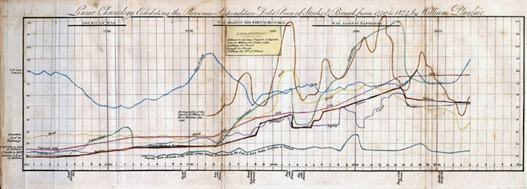
\includegraphics[scale=1]{images/historyOfGraphs}
\caption{Az egyik első statisztikai gráf (forrás: \cite{oldGraph})}
\end{figure}

\SubSection{Grafikon típusok \cite{graphTypes}} 

\subsubsection{Vonaldiagram}

A vonaldiagram olyan grafikon, amely vonalakat használ az egyes adatpontok összekapcsolására. A vonaldiagram kvantitatív értékeket jelenít meg egy meghatározott időintervallumban. A pénzügyekben a vonaldiagrammokat általában egy eszköz vagy értékpapír történelmi árfolyamműveletének ábrázolására használják. 

	Működését tekintve egy vonal köti össze az egyes adatpontokat, amelyek jellemzően mennyiségi értékeket jelenítenek meg. Befektetések terén a technikai elemzés területén a vonalgrafikonok meglehetősen informatívak, lehetővé téve a felhasználó számára a trendek megjelenítését. Míg a vonaldiagrammokat sok különböző mezőben használják különböző célokra, leggyakoribb funkciójuk az értékek időbeli változásainak grafikus ábrázolása.

\begin{figure}[h]
\centering
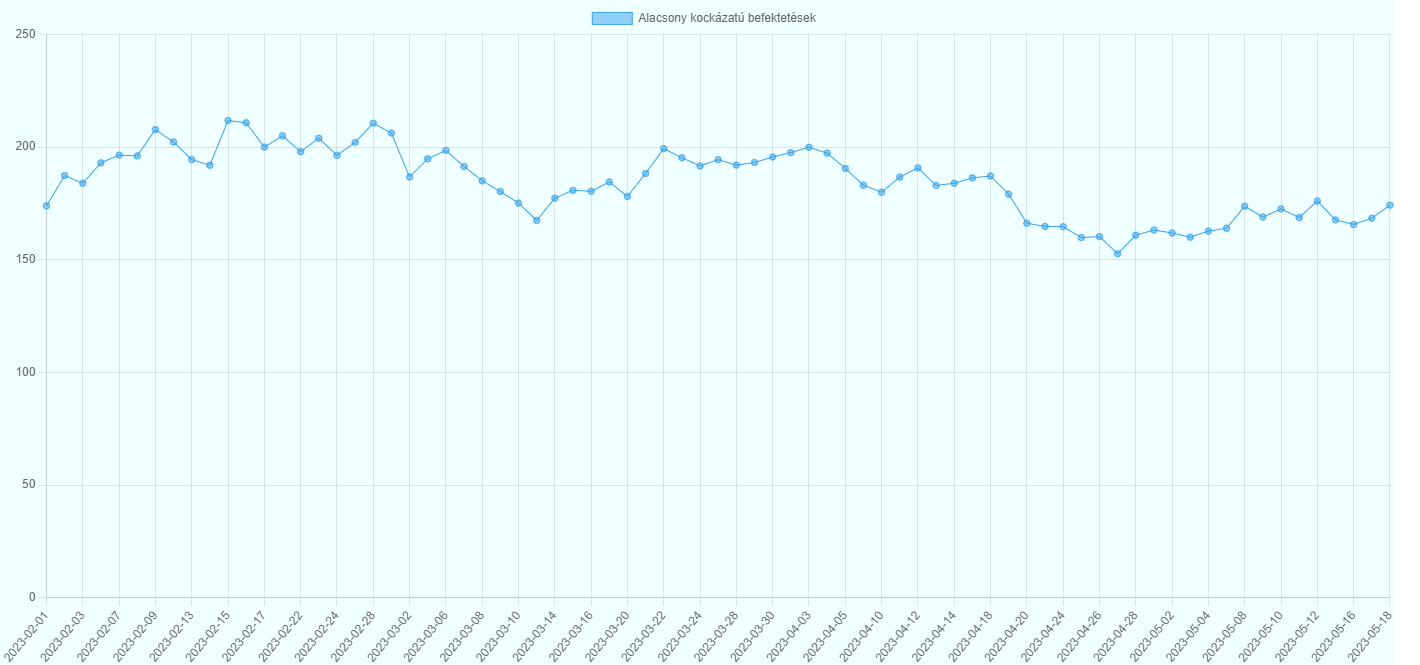
\includegraphics[scale=0.3]{images/lineChartExample}
\caption{Általam készített grafikonrajzoló oldalán megjelenített vonaldiagram}
\end{figure}

\subsubsection{Oszlopdiagram}

Az oszlopdiagram az információ grafikus ábrázolására szolgál. Különböző magasságú sávokat használ az értékek kimutatására. 

	Működését tekintve oszlopdiagrammokat létre lehet hozni függőleges sávokkal, vízszintes sávokkal, csoportos sávokkal (több sáv, amelyek egy kategória értékeit hasonlítják össze) vagy halmozott sávokkal (több típusú információt tartalmazó oszlopok). A sávok egy adott adatkategória értékét jelenítik meg az hatázorra meg annak méretét. Az oszlopdiagramokat általában az üzleti és pénzügyi elemzésekben használják a gyakran bonyolult adatok megjelenítésére, mivel gyorsan és hatékonyan tudnak információt közvetíteni.

\clearpage

\begin{figure}[h]
\centering
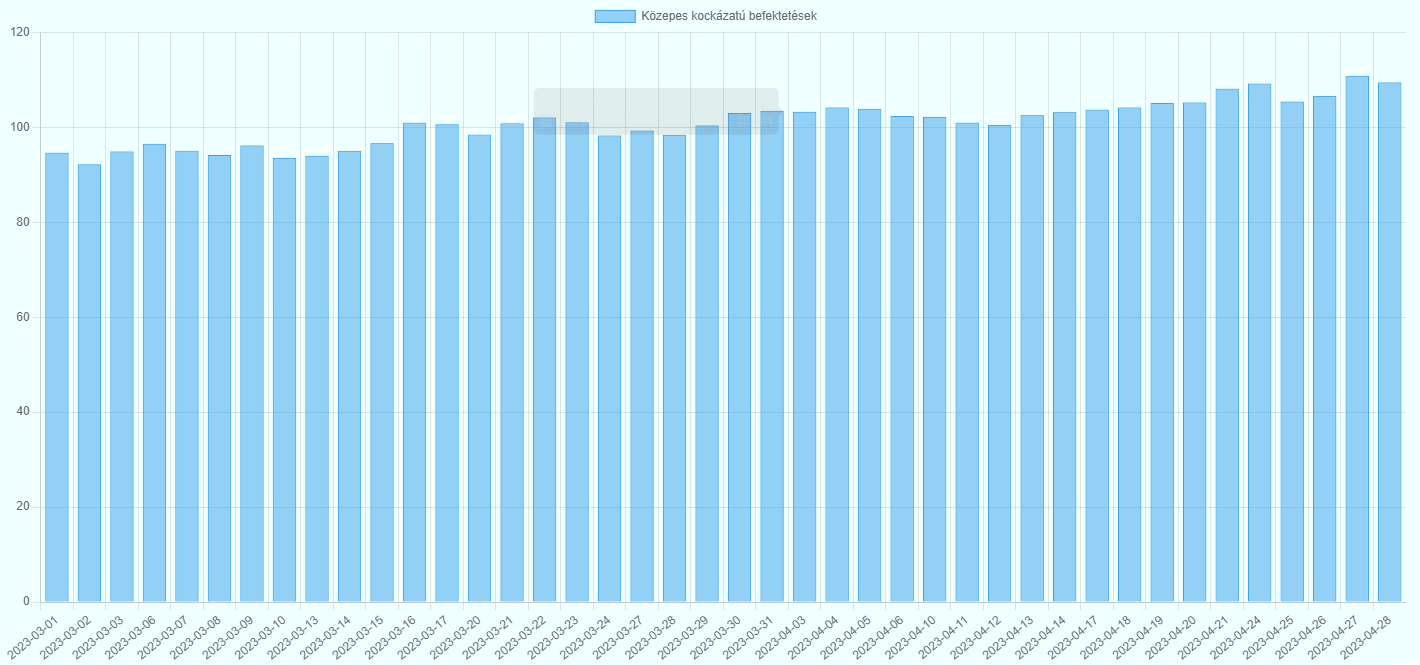
\includegraphics[scale=0.3]{images/barChartExample}
\caption{Általam készített grafikonrajzoló oldalán megjelenített oszlopdiagram}
\end{figure}

\subsubsection{Kördiagram}

A kördiagram egy névleges adathalmaz összegzésének vagy egy adott változó különböző értékeinek megjelenítésének módja (pl. százalékos eloszlás). A kördiagrammok használata meglehetősen népszerű, mivel a kör vizuális koncepciót ad az egészről. Egyik alfaja a poláris diagram.

	Működését tekintve az ilyen típusú diagram egy szegmenssorozatra osztott kör. Minden szegmens egy adott kategóriát képvisel. Az egyes szegmensek területe a körnek ugyanolyan arányban van, mint a kategória a teljes adatkészletben.

\begin{figure}[h]
\centering
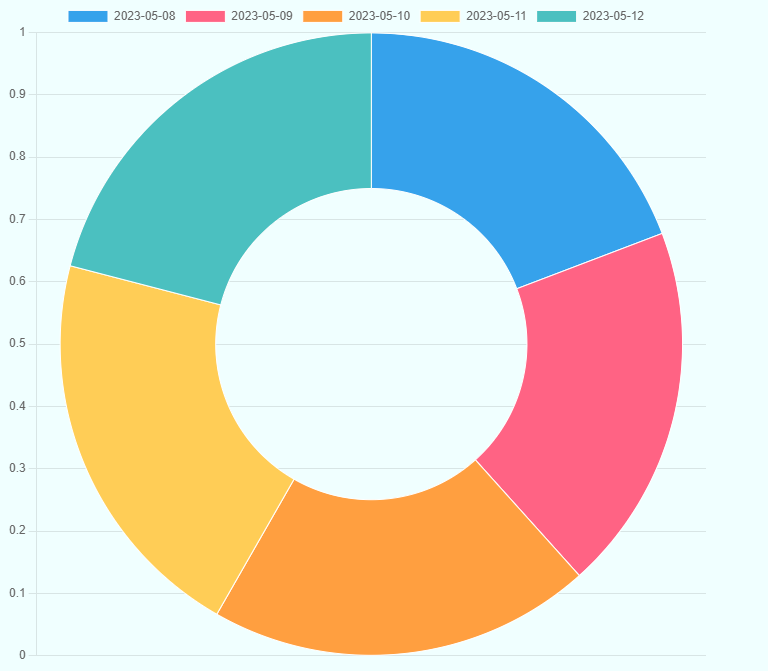
\includegraphics[scale=0.4]{images/pieChartExample}
\caption{Általam készített grafikonrajzoló oldalán megjelenített kördiagram}
\end{figure}

\subsubsection{Radardiagram}

A radardiagram segít szemléltetni a különböző jellemzőkkel rendelkező adatcsoportok összehasonlítását. Segítségével könnyen össze lehet mérni másfajta paraméterekkel rendelkező elemeket. 

	Működését tekintve az adatokat ugyanarra a központi pontra helyezi, és átlátszó árnyalatokkal és mintákkal mutatja be a kontrasztot az olvasó számára. Egy adott pont értékének nagyságát az jelzi, minél távolabbra nyúlik az origótól a pókháló szerű diagrammon.

\begin{figure}[h]
\centering
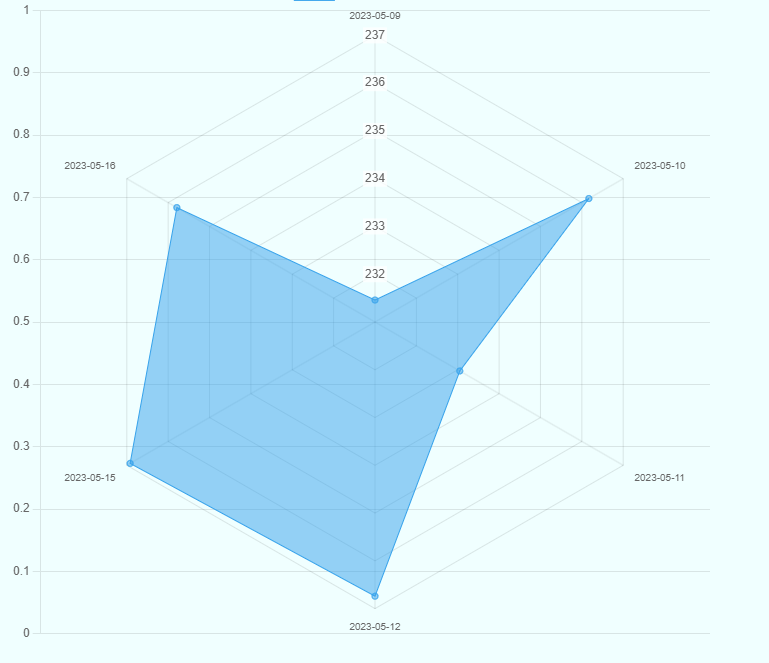
\includegraphics[scale=0.4]{images/radarChartExample}
\caption{Általam készített grafikonrajzoló oldalán megjelenített radardiagram}
\end{figure}

\Section{Tőzsde}

A tőzsde talán a modernt világ egyik legjobban félreértelmezett kifejezése.A hétköznapi ember lelki szemei előtt számok végtelen sokasága lebeg, amikor meghallja és csak legyint rá, hogy ez számára túl komplikált, ahhoz, hogy átlássa és megértse. Nos, ez az állítás részben igaz is, hiszen lehet nagyon bonyolult a tőzsde, viszont lehet nagyon egyszerű is.

	A tőzsde egy olyan nyilvános, központosított és szervezett piac, ahol meghatározott árukat, meghatározott időben, azon belül meghatározott személyek adhatnak, vagy vehetnek szigorú eljárási szabályok szerint.  Ez mit is jelent a gyakorlatban? A tőzsde is egy olyan piac, mint amilyet akármelyik városban, vagy faluban találhatunk. A különbség az, hogy vásárlás során maga az áru nem materiális formában jelenik meg, illetve nem csak az adott környezettel, hanem az egész világgal lehetőségünk van kereskedni. Viszont, hogy mibe érdemes fektetni az bonyolultabb, mint elsőre képzelnénk.  \cite{wikiStock}
	
A tőzsdék fajtái lehetnek: 

\begin{itemize}
\item Árutőzsde
\item Értéktőzsde, ezen belül: 
	\begin{itemize}
	     \item Devizatőke
	     \item Értékpapírtőzsde 
	     \item Hírpiac
	\end{itemize}
\end{itemize}

\SubSection{Részvény}

A részvény tulajdonjogot és egyéb gazdasági jogokat megtestesítő értékpapír, nincsen lejárati ideje. Ezeket az értékpapírokat a részvénytársaságok a részvény birtokosainak, annak részesedése arányában osztják szét jövedelem és szavazati jogok arányos formájában.

	A részvények nagyobbrészt névre szóló értékpapírok, amelyeket leginkább elektronikus úton, dematerizált formában állítanak elő, hogy kereskedelmi forgalomba hozhatóak legyenek. A fizikai értékpapírok tárolása leginkább bankokban, vagy takarékszövetkezetekben történik. A részvényekkel tőzsdén kívüli piacokon is kereskednek, amelyekre általában lazább szabályok vonatkoznak, mint a központosított piacokon. 

	A részvénytulajdonlás jövedelem növelése érdekében történik. Egy vállalat termelő, vagy szolgáltató tevékenységének célja a profitszerzés, hogy ezt elérhetővé tegye részvénytársasággá kell vállalnia. A vállalkozásban lévő részesedést az alapító tagok között szokás meghatározni, hogy mely tag mekkora összeggel járult hozzá az adott vállalkozás elindításához. Abban az esetben, ha csak az alapítók rendelkeznek részesedéssel, akkor zárt részvénytársaságról beszélünk. Amennyiben az alapítók úgy határoznak, hogy a céget a nyilvánosság elé tárják, akkor zártkörű helyett a cég elkezd részvényeket kibocsájtani. Ezen részvények összessége arányos azzal a tulajdonjoggal, amiről az alapítók lemondtak.

	Többfajta részvénytípusok elérhetőek, a teljesség igénye nélkül felsorolok párat, például: befektetési életbiztosítások, \textbf{befektetési alapok}, nyugdíj célú megtakarítások.  \cite{wikiShare}

\Section{Befektetési alapok}

Azon személyek, akik pénzüket beszerették volna fektetni valamilyen szolgáltatásba, már nagy eséllyel hallottak a befektetési alapokról. Ezen termékek kedvezőek és meggyőzőek lehetnek bárki számára. A tőzsde egyik „alapszabálya”, hogy befektetéskor nem ajánlott egyetlen terméket vásárolni. A diverzifikáció ugyanis nagyon fontos, hiszen nem csak ezzel csökkenthetjük a kockázatot, hanem sokkal több tapasztalatot is tudunk gyűjteni és minél több csapot nyit meg a befektető annál nagyobb eséllyel lesz sikeres. \cite{wikiInvest}

	A befektetési alap olyan vagyontömeg, amely állhat értékpapírból, ingatlanokból, bankbetétekből és részvényekből. Befektetési alapot csakis befektetési alapkezelő hozhat létre és kezelhet. Egy befektetési alapkezelő több befektetési alapot is kezelhet. A befektetési alapok futamideje változó, beszélhetünk akár pár hónapos futamidőről, de akár évtizedekig tartó időintervallumról is. A rövid futamidejű alapokat likvidálási alapoknak hívjuk és mindig nyitott végű alapok. Mit jelent az a kifejezés, hogy \emph{nyitott végű alap}ok? 

	A befektetésí alapokat két fajta típus alapján különböztetjük meg, ezen típusok jelzik, hogyan lehet csatlakozni egy alaphoz.
\begin{itemize}
\item \textbf{Nyíltvégű alapok}: bármelyik forgalmazási napon lehetőségünk nyílik csatlakozni, illetve vissza is válthatjuk belőle a megtakarításainkat. Ezek az alapok általában határozatlan futamidőre jönnek létre és mi dönthetjük el, meddig tartjuk bent a megtakarított pénzünket. Mindig érdemes figyelni a javasolt befektetési időtávokat, hogy a befektetésünk jó eséllyel az elvárt teljesítményt tudja nekünk szolgáltatni.
\item \textbf{Zártvégű alapok}: a zártvégű alapokhoz csak az alap indulása előtti jegyzési időszakban van lehetőségünk csatlakozni. Ezen alapok általában határozott futamidőre jönnek létre, tehát az alap lejárattal rendelkeznek, ezen időszakig a megtakarításainkat az alapban kell tartanunk. Természetesen, ha a futamidő alatt mégis szükségünk lenne a befektetett összegre, a zártvégű alapokat tőzsdei megbízás útján értékesíteni tudjuk, ilyenkor a pillanatnyi kereslet fogja meghatározni a befektetésünk ellenértékét, nem pedig annak az értéke. Ezért, fontos jól megfontolni, ha zártvégű alapot választunk, célszerű és javaslott a befektetésünket a lejáratig megtartani.  

Az alapokat az alapján is csoportosíthatjuk, hogy azok milyen típusú eszközbe fektetik a befektetők megtakarításait.  

\end{itemize}
\begin{itemize}
\item \textbf{Pénzpiaci befektetési alap}: pénzpiaci alapok, állampapírok és különböző banki betétek.
\item \textbf{Kötvényalapok}: különböző kötvények vásárolhatók.
\item \textbf{Részvényalapok}: vállalatok által kibocsátott részvények.
\item \textbf{Vegyes alapok}: többféle portfólióban csoportosított részvények és  kötvények.
\item \textbf{Ingatlan befektetési alap}: már megépült vagy építésben levő ingatlanokba való befektetés.
\item \textbf{Speciális befektetési alapok}: abszolút hozamú, tőkevédett és származtatott alapok. \cite{OTPInvest}
\end{itemize}

	Mivel ilyen sokrétű lehet egy befektetési alap, így felmerülhet a vásárlóban, hogy miért érdemes befektetési alapba fektetnie a pénzét? Erre a kérdésre az egyik legjobb érv a kockázatmegosztás. Ugyanis már egyetlen befektetési alap megvásárlásával is több egyedi értkékpapírból álló, szakszerűen összeállított portfólióhoz juthatunk hozzá, amit egyéni befektetőként rengeteg idő és erőfeszítés árán révén érhetnénk el. Amennyiben befektetési alapot választunk megtakarításaink elhelyezésére nincsen más dolgunk, mint vásárolni az alap befektetési jegyeiből. Ezzel az egyszerű tranzakcióval gyakorlatilag megbízunk egy szakértői gárdát, akik az összes a befektetésünkkel kapcsolatos terhet levesznek a vállunkról, és különféle értékpapírokba helyezik el megtakarításaikat.

\begin{figure}[h]
\centering
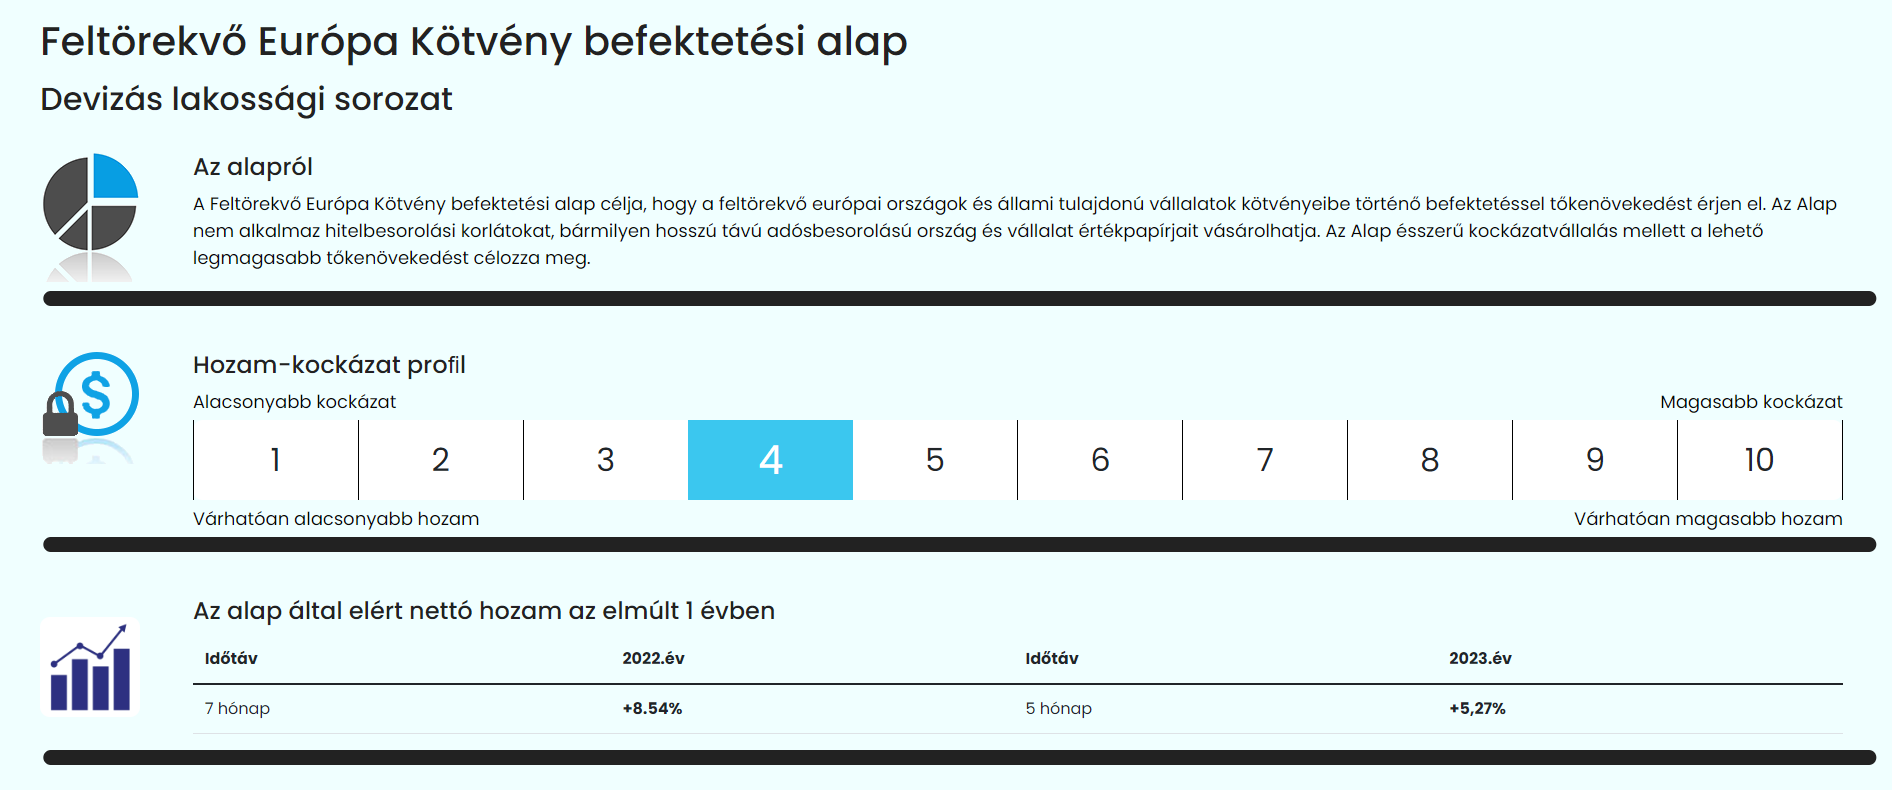
\includegraphics[scale=0.3]{images/europeInvestExample}
\caption{Általam készített weboldal egyik befektetési alapja}
\end{figure}

\SubSection{Tőzsdei árfolyam }

Tőzsdei árfolyamoknak nevezett árfolyamokat a globális pénzügyi piacon határozzák meg, ahol a bankok és más pénzügyi intézmények éjjel-nappal kereskednek valutákkal ezen tényezők alapján. Az árfolyamot általában az általa képviselt nemzeti valuta betűszóval jegyzik, mint például a leggyakrabban használt valuta az \emph{USD}, ami az amerikai dollárt jelenti. Mérésének számos módja van, a  leggyakoribb módszer a kétoldalú árfolyam mérése. A bilaterális árfolyam az egyik valuta másikhoz viszonyított értékére vonatkozik. A tőzsdén található árfolyamoknak több típusát különböztetjük meg, ezek az alábbiak lehetnek: 
\begin{itemize}
\item Nyitó árfolyam
\item Napi maximum érték
\item Napi minimum érték
\item Napi záró érték
\item Napi átlag érték \cite{exchangeRate}
\end{itemize}


\Chapter{Specifikáció}

Az előző fejezetben taglaltam milyen fogalmakkal találkozhat a felhasználó a weboldalon. Ebben a fejezetben ismertetem a szoftver tervezésének lépéseit, a felhasznált technológiák technikai hátterét, továbbá bemutatom az általam válaszott grafikus könyvtárat a Chart.JS-t és hogy miért erre esett a döntésem.

\section{Tervezés  \label{fig:planning}}

A programom tervezése során több szempontot vettem figyelemben. Elődleges szempont volt, hogy webalkalmazásként működne legjobban. Ezt az érvet azzal tudom alátámasztani, hogy szem előtt tartva az előnyeit (könnyű hozzáférés, naprakész adatok, jól szemléltethető, skálázható), illetve személyes szakmai tudásomat is a frontend fejlesztés során szereztem. Másodlagos érvemet pedig azzal tudom alátámasztani, hogy az egyetemi tanulmányaim során is webfejlesztésre szakosodtam.

	Az alkalmazás tervezésekor az egyik általam ismert agilis módszertan szerint dolgoztam, amelynek neve \emph{Extreme Programming} (XP). Az Extreme Programming egy specifikus keretrendszer, amelynek célja nem csak a kiváló minőségű szoftver(ek) előállítása, hanem az egész folyamat megkönnyítése is a fejlesztő számára.  A fejlesztési folyamatomatot 5 fázisra lehet bontani.\cite{agile} \\

\textbf{Tervezés (planning)}
\begin{itemize}
\item Piackutatás
\item Funkciók meghatározása
\item Szerver-kliens architektúra megtervezése
\item Felhasználandó technológiák
\end{itemize}

\textbf{Elemzések (analysis)}
\begin{itemize}
\item Alkalmazás struktúrákra felosztása
\item Elkészüléshez szükséges idő meghatározása
\item Szakmai tudás felmérése
\item Erőforrás tervezés fejlesztői oldalon
\end{itemize}

\textbf{Design}
\begin{itemize}
\item A feladatok lebontása
\item Összpontosított megjelenés létrehozása és végrehajtása
\end{itemize}

\textbf{Végrehajtás (execution)}
\begin{itemize}
\item Kódolás
\item Kész egységek tesztelése
\item Hibajelentés generálása
\item Iteráció közbeni és végi áttenkintés
\item Folyamatfejlesztések
\end{itemize}

\textbf{Zárás (closure)}
\begin{itemize}
\item Az elkészült termék üzembe helyezése
\item Felhasználói kézikönyv
\item Végső tesztelés
\end{itemize}

\section{Felhasznált technológiák}

\subsection{HTML5}
Mivel a programom online felületre lett tervezve, annak szerkezeti felépítése HTML-ben íródott. A HTML azaz Hypertext Markup Language, magyarul hipertext jelölő nyelv, egy leíró nyelv, amely egy weblap felépítését specifikálja az internetes böngészők felé. Ahogy nevében is láthatjuk, nem egy programozási nyelv, ez azt jelenti, hogy nem programozási logikák megírására, vagy adatok kezelésére használjuk, hanem különböző utasításokkal meghatározzuk az oldalunk struktúráját. \\

\begin{figure}[h]
\centering
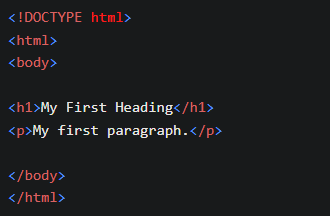
\includegraphics[scale=0.8]{images/htmlExample.png}
\caption{HTML felépítés és elemek megjelenítése}
\end{figure}

\subsubsection{HTML Canvas} 

Canvas elem a HTML5 része és lehetővé teszi két dimenziós alakzatok és dinamikus bittérképek megjelenítését. Több elterjedt 2D API-khoz hasonló rajzfunkciók teljes készletén keresztül érheti el a felhasználni kívánt területet, ezzel elérhetővé téve a dinamikusan generált grafikákat. Főbb felhasználási területe: grafikonok, animációk, játékok és képalkotás.

Mivel grafikonok megvalósításához elengedhetetlen, ezért az én applikációm részét is képezi. A Canvas elem a következőképpen épül fel:
\begin{figure}[h]
\centering
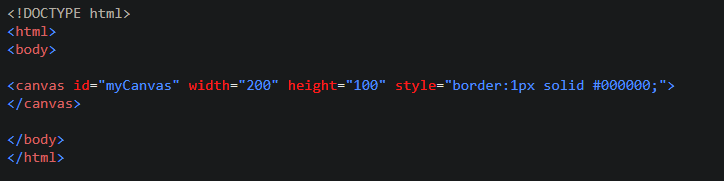
\includegraphics[scale=0.7]{images/canvasExample.png}
\caption{Egy üres négyzet, megvalósítva Canvas elem által}
\end{figure}

\subsection{CSS}

Ahhoz, hogy a HTML által definiált oldalunkon megjelenjenek a kívánt elemek és ezeket jól olvashatóan és igényesen tudjuk megformázni, szükségünk van egy olyan nyelvre, ami a HTML elemekre tud hivatkozni, és különböző nézeti tulajdonságokat tud neki átadni. Ezen célra alkalmas a CSS azaz Cascading Style Sheets, magyarul lépcsőzetes stíluslapok, egy leíró nyelv, amely a HTML elemek megjelenítését, azok stílusát (például: elhelyezkedés, betűszín, karakter formátumok stb.) írj a le a böngésző számára. 

	Különböző választókkal jelölhetünk ki elemeket, azok nevére, osztályára vagy típusára hivatkozva. A lépcsőzetesség arra utal, hogy mely választók vannak priorizálva a weblap megjelenítésének szempontjából. Ez fontos, hisz összetett weblapok esetén többszáz CSS szabály is használatban lehet. \newline
	CSS stílusokat megadhatunk különféle eljárások szerint. \aref{fig:css} \\

	Közvetlenül egy HTML elemen keresztül pontosvesszőkkel elválasztva. Ezt a változatot \emph{sorközi stílus}nak (inline CSS) nevezzük. \\

	Használhatjuk \emph{belső stílus}ként (internal CSS), amely egyedi kinézetet biztosít egyetlen dokumentumhoz. A HTML <head> részében kell meghatározni <style> címkén belül. \\

	Szakmailag legelterjedtebb felhasználása a \emph{külső stílus} (external CSS). A külső stíluslapot általában akkor használjuk, ha több oldalon szeretnénk változtatni. Ideális erre az állapotra, mert megkönnyíti a teljes webhely megjelenésének megváltoztatását egyetlen fájl módosításával. Fejrészen belül elhelyezzük <link> címkék közé a külső fájl forrását, amiben a kódunk szerepel.

\begin{figure}[h]
\centering
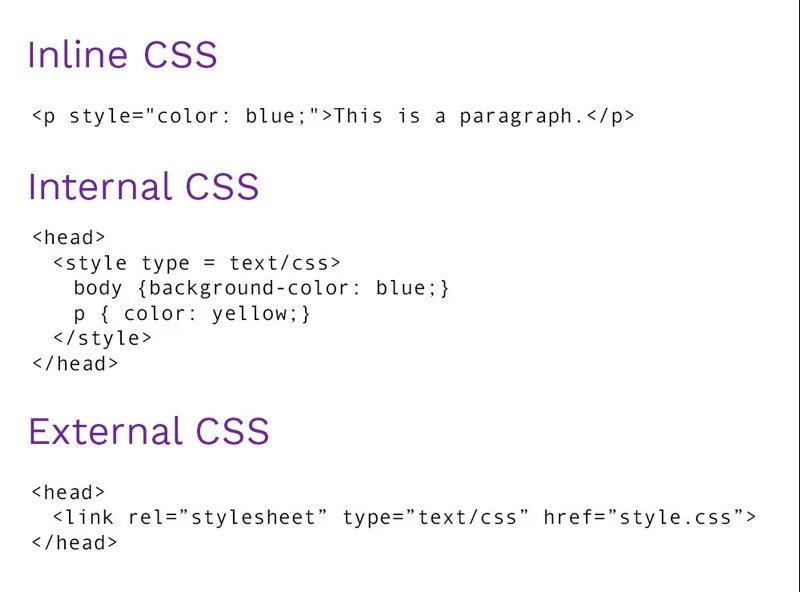
\includegraphics[scale=0.5]{images/cssTypes.png}
\caption{Különböző CSS elérési útvonalak. (forrás: \cite{cssTypes})}
\label{fig:css}
\end{figure}

\subsubsection{Bootstrap5}

A Bootstrap egy ingyenes, nyílt forráskódú frontend fejlesztői keretrendszer webhelyek és webes alkalmazások létrehozásához. Úgy tervezték, hogy lehetővé tegye a webhelyek reszponzív fejlesztését , és a Bootstrap szintaxis gyűjteményt biztosít a sablontervekhez, így a fejlesztőknek csak be kell illeszteni a kódot egy előre meghatározott CSS-keretrendszerbe (grid). Ez a rendszer 12 oszlopos rácsrendszert használ, ezáltal egy reszponzív weboldalt több módon egyenletesen lehet felosztani, ahogy az eszköz nézete megváltozik különféle felbontásban. \cite{Bootstrap}

\begin{figure}[h]
\centering
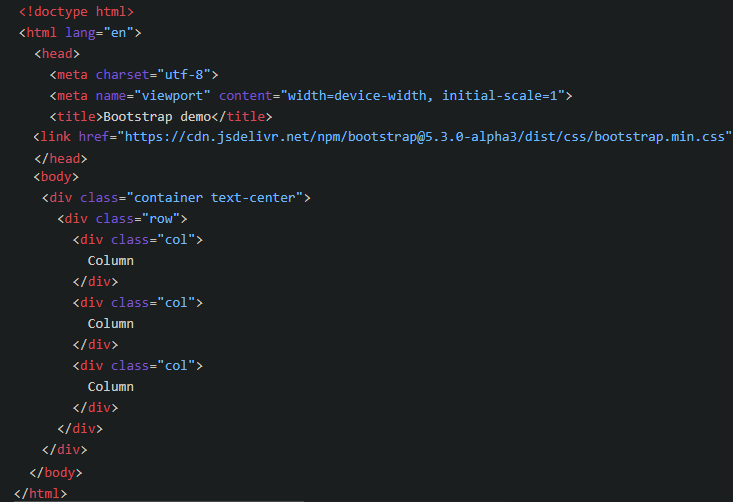
\includegraphics[scale=0.5]{images/bootstrap.png}
\caption{Bootstrap beillesztése HTML dokumentumban és rácsrendszer felosztása }
\end{figure}

\paragraph{Rácsrendszer:}

A rácsrendszerek olyan segédeszközök, amelyeket a tervezők a nehezen átlátható weboldalak megoldásaként valósították meg, hogy az információk rendezettek legyenek és következetes felhasználói élményt biztosítsanak a felhasználók számára. Logikáját tekintve szakított az informatikában gyakran használt decimális számokkal, mivel ezen számokat nem lehet felezni, harmadolni, úgy, hogy egész számokat kapjunk. Így merült fel az a meglátás, miszerint a tároló konténert 12 egyenlő részre osztja fel. Szabadon beállíthatjuk az adott sor(ok), vagy oszlop(ok) milyen szélességgel rendelkezzenek, esetleg a tároló kontéren mekkora részének feleljen meg a képernyőn.

\begin{figure}[h]
\centering
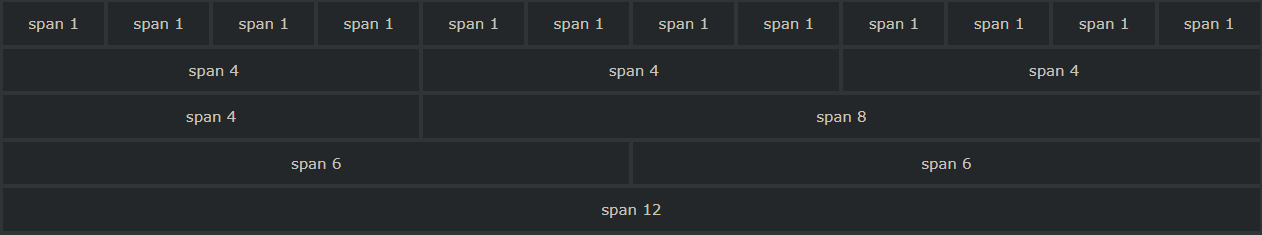
\includegraphics[scale=0.4]{images/gridSystem.png}
\caption{12 oszlopos rácsrendszer felosztása (forrás: \cite{gridSystem})}
\end{figure}

\subsubsection{Font Awsome}

A legegyszerűbb módja annak, hogy figyelemfelkeltő ikonokat helyezzünk el weboldalunkon, ha ikon készletet használunk. Én a Font Awsome internetes ikonkönyvtárát és eszközkészletét használtam fel.

\subsection{NodeJS }

A Node.js egy nyílt forráskódú, többplatformos futási környezet amiben a gépünkön JavaScript kódot tudunk végrehajtani. Széles körben használják szerveroldali programozáshoz, így a fejlesztők használhatják a JavaScriptet kliensoldali és szerveroldali kódokhoz anélkül, hogy további nyelvet kellene megtanulniuk. Általában egy bizonyos címen és porton figyel az szerver, és mikor kérést kap, elvégzi a leprogramozott funkciókat, majd tétlen állapotban várakozik a következő hívásig. Mivel a Node.js nem folytat közvetlenül kimeneti, vagy bementi műveleteket, így erőforrások blokkolása nem merül fel, ezáltal nem kell félni, hogy a program elakad. Tehát a Node.js ideális interaktív megjelenítő alkalmazások fejlesztésére. \cite{nodeJS}

\subsubsection{Node Package Manager}

A Node.js futtatásához Node Package Manager (NPM), azaz Node Csomagkezelőt alkalmazunk. Az NPM egy nyílvántartott adatbázis, amelyben szotfverek és a hozzájuk található metaadtok szerepelnek. Három részre lehet felosztani, úgy mint weboldal kezelés, parancssori felület és nyilvántartás.

\subsubsection{Express.JS}

Az Express.js egy Node.js backend keretrendszer, amelyet arra terveztek, hogy az API webalkalmazásait gyorsan és platformokon átívelő almazásokat készítsen, és megkönnyítse a node js-t dolgát. Webes alkalmazások és RESTful API-k építésére tervezték anélkül, hogy bármiben is korlátozná a szerver funkcióit.

\subsection{JavaScript}

A JavaScript, amelyet gyakran JS-ként is szoktak említeni, egy olyan többparadigmás, dinamikus programozási nyelv, ami lehetővé teszi, hogy a weblapokon komplex funkciókat valósíthassunk meg HTML és CSS használatával. A webhelyek majdnem 100\%-a JavaScriptet használ az elsőrendű függvényeivel, továbbá az alacsony erőforrásigényével. Támogatja a prototípus-alapú objektumorientációval és első osztályú funkciókkal rendelkező kódolást, továbbá az eseményvezérelt, funkcionális és kötelező programozási stílusokat. 

Működését tekintve, nem típusos nyelv, így nem szükséges a változókat deklarálni használat előtt, a megfelelő típust futás közben veszi fel. A JavaScriptet támogató böngésző betölti a HTML oldalt, amennyiben script kód található benne a JavaScript elemző motor kerül előtérbe és a script kód betöltődik. Alkalmazásprogramozási felületekkel (API-kkal) rendelkezik a szöveggel, dátumokkal, reguláris kifejezésekkel való munkához. A legnépszerűbb futásidejű rendszer erre a felhasználásra a Node.js. \\
(Bár a Java és a JavaScript nevüket és szintaxisukat tekintve hasonlóak, a két nyelv különbözik, és nagymértékben eltér egymástól.)  \cite{wikiJS}


\subsubsection{JQuery}

A jQuery egy nyílt forráskódú, gazdag JavaScript-keretrendszer, amely leegyszerűsíti a HTML/CSS-dokumentumok, pontosabban a Dokumentum Objektum Model (DOM) és a JavaScript közötti interakciókat. Szintaxisát úgy tervezték, hogy megkönnyítse a dokumentumban való navigálást, kezelést, a DOM- elemek kiválasztását, az animációk létrehozását, az események kezelését és az Aszinkron JavaScript XML (Ajax)- alkalmazások fejlesztését.

	 A jQuery lehetőséget biztosít, a fejlesztők számára, hogy absztrakciókat hozzanak létre alacsony szintű interakcióhoz és animációhoz, fejlett effektusokhoz és magas szintű, témára alkalmas widgetekhez. A könyvtár moduláris megközelítése lehetővé teszi hatékony dinamikus weboldalak és webalkalmazások létrehozását. \\

\subsubsection{JSON}

A JavaScript Objektum Jelölés (JSON) egy nyílt szabványos,  nyelvtől független fájlformátum és adatcsere -formátum, amely ember által olvasható szöveget használ az adatobjektumok tárolására és továbbítására. Nagyon elterjedt adatformátum, amelyet sokrétűen alkalmaznak az elektronikus adatcserében, beleértve az adatcserét webes alkalmazások és szerverek között. A JSON két struktúrára épül: \\

Név - érték párok gyűjteménye. Különböző nyelveken ez objektumként , rekordként, struktúraként, szótárként, hash-táblaként, kulcsos listaként vagy asszociatív tömbként valósul meg .Az értékek listája rendezett. Ezen értékek lehetnek, sztringek, számok,  másik JSON, tömbök, vagy boolean értékek. A .json fájlnevet ezen objektumok kiterjesztésére használják, nem csak JavaScript programozási nyelven íródott kódokra is. \\

\begin{figure}[h]
\centering
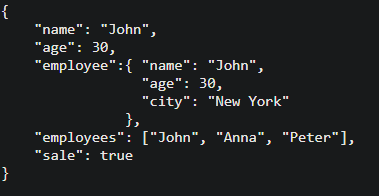
\includegraphics[scale=0.9]{images/jsonExample.png}
\caption{Egy alkalmazott adatai JSON-ként tárolva }
\end{figure}


\section{Miért a Chart.JS? }

\subsection{ChartJS bemutatása}

A Chart.js egy ingyenes, nyílt forráskódú JavaScript-könyvtár adatvizualizációhoz , amely nyolc diagramtípust támogat : vonal, oszlop, terület, torta ( fánk ), buborék, radar, poláris és szórt diagram. JavaScript nyelven használt beépülő modulokat, diagramtípusokat és testreszabási lehetőségeket kínál. A számtalan beépített modul mellett, a közösség által karbantartott diagramtípusokat is elérhetővé tesz. Ezen felül több diagramtípus kombinálható vegyes diagrammá ugyan azon a Canvas elemen belül. \cite{ChartJS}

\begin{figure}[h]
\centering
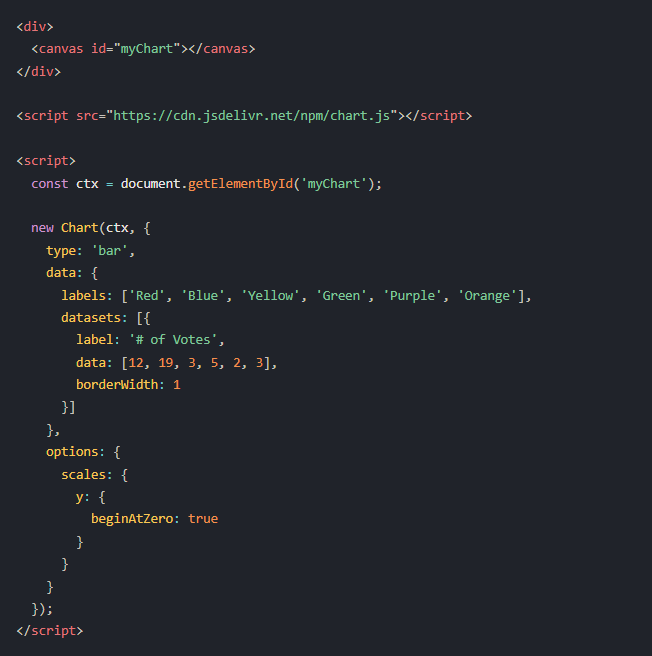
\includegraphics[scale=0.6]{images/chartExample.png}
\caption{diagram létrehozása JSON formátumban (forrás: \cite{ChartJS})}
\end{figure}

\begin{figure}[h]
\centering
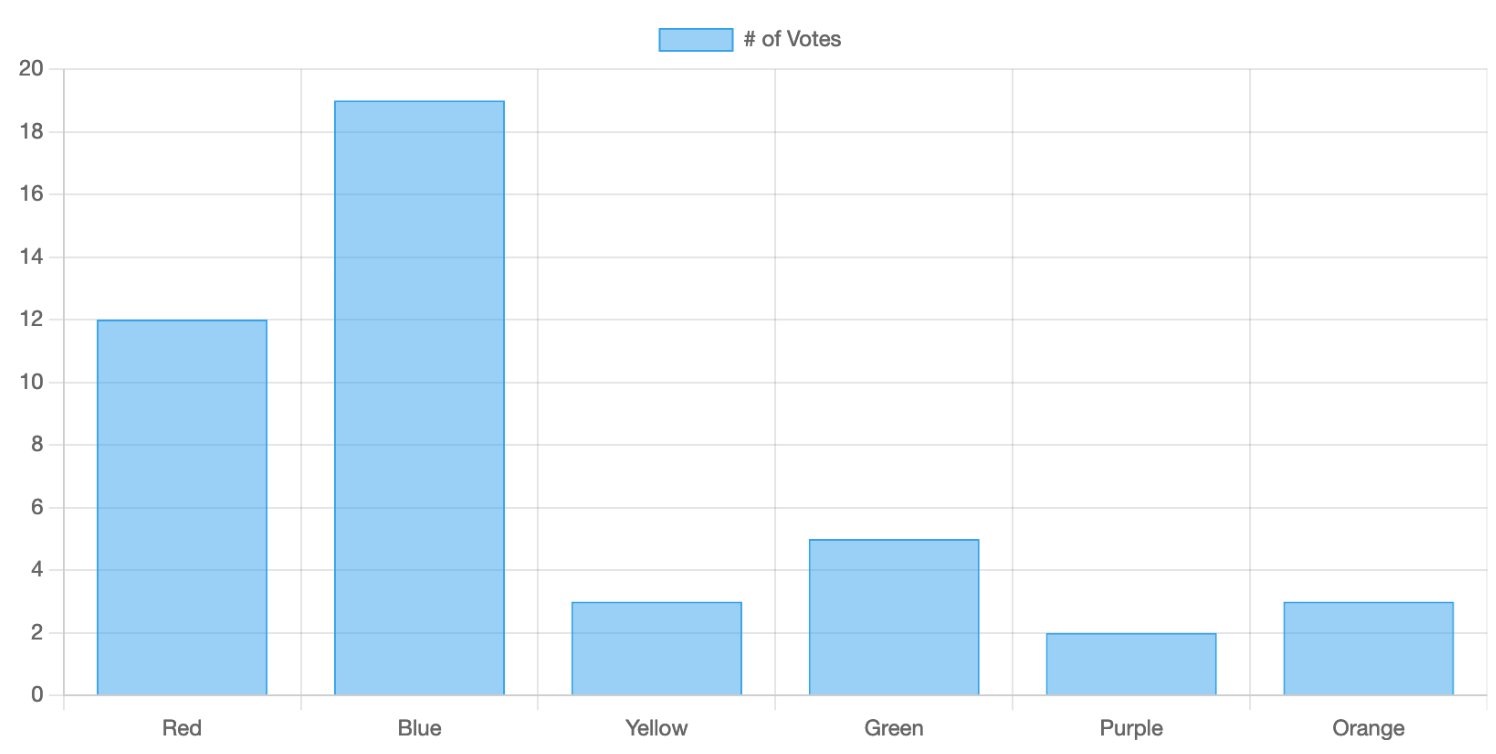
\includegraphics[scale=0.3]{images/barChartJSExample.png}
\caption{Oszlopdiagram ami szavazatok számát mutatja meg (forrás: \cite{ChartJS})}
\end{figure}

\subsection{ChartJS összehasonlítása más grafikus könyvtárakkal}

\subsubsection{Chart.JS összehasonlítása D3.JS keretrendszerrel}
A csillagok száma alapján a GitHubon a második legnépszerűbb JavaScript diagramkönyvtár a D3.js után, amelyet ugyan lényegesen könnyebben használhatónak tartanak, de kevésbé testreszabható, mint az utóbbi. A Chart.js HTML5 Canvas elemen belül jelenik meg, és széles körben elismert, mint az egyik legjobb adatvizualizációs könyvtár.
A Chart.js nagymértékben testreszabható, hogy néhányat említsek: egyéni beépülő modulokkal, amelyek segítségével megjegyzéseket, nagyítást vagy húzással hozhat létre, hogy néhány dolgot említsünk 

	A Chart.js a diagramelemeket HTML5 Canvas jeleníti meg, ellentétben számos más, többnyire D3.js-alapú diagramkönyvtárral, amelyek Skálázható Vektor Grafika (SVG)-ként jelennek meg. A Canvas megjelenítés nagyon hatékonyvá teszi a Chart.js-t, különösen nagy adatkészletek és összetett vizualizációk esetén, amelyek egyébként több ezer SVG-csomópontot igényelnének a DOM-fában. Ugyanakkor a Canvas renderelés nem engedélyezi a CSS stílust, ezért ehhez beépített opciókat kell használni, vagy különböző diagramtípusokaz kell létrehozni, hogy a kívánt gráfokat jelenjenek meg. 

	A Chart.js nagyon jól használható nagy adathalmazokhoz. Az ilyen adatkészletek hatékonyan feldolgozhatóak belső formátum használatával, így eredményes az adatok elemzéséhez és normalizálásához. Végül a Chart.js által használt Canvas megjelenítés csökkenti a DOM-fájának terhelését, míg az SVG-megjelenítéshez nagyon erőforrás igényes tud lenni. \cite{wikiChart}

\paragraph{ChartJS előnyei}

\begin{itemize}
\item Mivel a Chart.js egy JavaScript könyvtár, így lehetővé teszi, hogy bármilyen választott JS keretrendszerrel használjuk, mint például az Angular.js vagy a React.js..
\item Használata könnyű és minimális fejlesztési ismeretet igényel.
\item Nyílt forráskódú, így csak a meglévő könyvtárat kell felhasználni és nem a fejlesztőnek kell mindent felépíteni.
\item World Wibe Web Consortion (W3C) szabványt követi, így a használatához nincs szükség más böngészőhöz tartozó technológiára, vagy bővítményre.
\item Több megjelenítő eszközzel ellentétben 8 féle diagram megjelenítését engedélyezi.
\item Adatok hatákony manipulálását teszi lehetővé. Rendkívül gyorsan jelenik meg és saját animációkkal rendelkezik.
\item Kiváló dokumentációval van ellátva.
\end{itemize}

\Chapter{Implementáció}

A specifikáció alapján a felhasználó naprakész háttérinformációval rendelkezik a fejlesztési folyamattal és a szükséges technológiák ismeretével kapcsolatban. Ezen ismeretek megszerzésével ebben a fejezetben prezentálni fogom az elkészült alkalmazás látható és háttérmunkaként szolgáló programrészeit.


\section{Áttekintés}

A szakdolgozatom témája interaktív megjelenítő eszköz (ez esetben weboldal) pénzügyi adatok elemzéséhez. Ilyen szoftverekből különféle megvalósítást lehet találni az interneten, amelyeket nagyobb befektetői hátérrel rendelkező cégek működtetnek általában valamilyen pénzbeli szolgáltatás ellenében. Számomra elsődleges szempontot képviselt a szabad és pénzmentes felhasználás, a könnyű kezelhetőség, átláthatóság és sokszínűség, különösképpen a grafikont illetően. A már bemutatott Chart.js technológia nagyszabásű könyvtárának ismeretével megalkotott gráfok több lehetőséget is a felhasználó elé tárnak, mind megjelenés, mind adathalmazok terén. 

\subsection{Problémakör}

Ahogy az Áttekintésben felvázoltam több grafikonrajzoló és eszközkezelő weboldal létezik napjainkban. Ezen oldalakat vizsgálva feltűnt, hogy több megkötés árán tudtam hozzájutni a kívánt adatokhoz. Az egyik ilyen megkötéssel akkor szembesültem, amikor a grafikonrajzolóhoz nem engedett hozzáférni felhasználó nélkül. Mivel teljes mértékben piackutatás céljából vizsgálódtam nem tartottam fontos szempontnak felhasználó regisztrálását, így az oldal használatát a továbbiakban nem tudtam folytatni.

	Következő korlátozás amivel találkoztam, hogy ugyan a biztosítók által használt webhelyek részvények és portfóliók széles körű tárházával rendelkeznek, de jogi és piaci okokból kifolyólag korlátozott az adatbázisuk, hiszen más vállalatok termékeit nem híresztelhetik. Kutatásaim során meggyőződtem, hogy ezen adatok nyilvánosak az ügyfelek számára, tehát illusztrálásuk engedélyezett bármely kliens részére.

	Továbbiakban széles körű adatforrással rendelkező portálokat után keresgéltem és sikeresen találtam pár ilyen paraméterekkel rendelkező weboldalakat. Azonban túlnyomórészt idegen nyelven íródtak, ami globális szinten érthető megközelítés, viszont mint magyar anyanyelvű felhasználó ezt problémának éreztem. 

\subsection{Program működésének elve}

Pár szóban kifejtem az alkalmazás milyen felhasználói körnek hoztam létre első sorban. Alapvetően adatbányász, tőzsdei jelenléttel rendelkező vállalatoknak ajánlanám, hiszen korlátozás nélkül bővíthető az adathalmaz, ezáltal optimalizálható bármely piaci részre. Felépítésében fontos kulcsszerepet képviseltek az alábbi szempontok:

\begin{itemize}
\item \textbf{Megjelenés}: Felépítése, megjelenése letisztult és modern, jelképezve egy innovatív oldal behatását.
\item \textbf{Reszponzivitás}: Weboldalam célja, hogy optimális megjelenést biztosítson \\
(könnyű olvashatóság, egyszerű navigáció) a legkülönfélébb eszközökön az asztali számítógépektől egészen a mobiltelefonokig. Az oldal tökéletesen igazodik a megjelenítő eszközhöz a rugalmas felépítésével és flexibilis képeivel.
\item \textbf{Egységes színvilág}: Színvilág megvalósításánál elengedhetetlen tényező volt, hogy a felhasználónak kellemes színeket használjak, amelyek harmonizálnak egymással. Szubjektív kikötésem volt a fehér háttérszín elvetése, mert számomra szemvakító.
\item \textbf{Egységes formavilág}: Az egész weboldalnak egységes a formavilága, könnyen felismerhető panelekkel felépítve. A gombok, képek és szöveg megjelenése nem tér el panelenként szemben sok más alkalmazással.
\item \textbf{Navigálhatóság}: A weblap összes panele könnyen elérhető akár a navigációs sáv használatával, akár az oldalak közti kommunikációval.
\item \textbf{Funkciók}: Implementált funkciók szerepüket működésük szerint betöltik, bármely böngészőn futtatjuk az alkalmazást.
\item \textbf{Tartalom}: Releváns és minőségi értéket ad a látogató számára.
\item \textbf{Honlapszerkezet}: Az oldalak hierarchikusan vannak felépítve, tehát logikusan következnek egymásból.
\end{itemize}

\section{Fejlesztési eszközök}

\subsection{Részvények adataihoz való hozzáférés}

A részvények adatainak az igénybe vételét külsős oldal segítségével oldottam meg. Az oldal amit használok az \emph{EOD Historical Data}, amely egyszerű hozzáférést biztosít az alapvető tőzsdei adatokhoz és az országokból származó részvényekhez és befektetési alapokhoz. Az oldalon található adatok védettek, ezért egy biztonsági eljárás útján tudom elérni őket. Ezen eljárás alapján a regisztrált felhasználómhoz az oldal generál úgy nevezett "API KEY"-t, ami minden felhasználónak egyedi és elengedhetetlen része az adatokat lekérő URL-nek. Miután megszereztem az kulcsot a lekérdezésben feltétlenül szerepelnie kell, különben nincs jogosultságunk az adatok eléréséhez.  \cite{eod} \\

\begin{figure}[h]
\centering
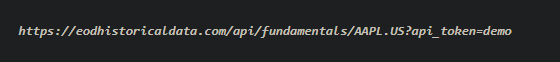
\includegraphics[scale=0.9]{images/demoAPI.png}
\caption{API hívás demo ID-val (forrás:\cite{eod})}
\end{figure}

\pagebreak
	Elérhető fizetős és ingyenes változata is, én az utóbbit használom, amivel némi megkötéssel kellett szembesülnöm, mint például a maximum időintervallum amira az API-hívások szólhatnak az 1 év, tehát a grafikon ábrázolásának van határa. Illetve naponta csak 20 hívást tudok intézni, így egy erre a problémára egy megoldással kellett előállnom, amit a \aref{fig:server} \textbf{Szerver} szekcióban fogok ismertetni.

\subsection{Postman}

Mivel nem készült adatbázis az alkalmazásomhoz, így a fenti részben említett API hívásokat külső applikációval valósítom meg, ez pedig a \emph{Postman}. A Postman az egyik legnépszerűbb szoftvertesztelő eszköz, amelyet API tesztelésre, létrehozására, megosztására és dokumentálásra alkalmaznak a fejlesztők. 

	Működését tekintve igen egyszerű a használata (lásd: \aref{fig:postman}). Elsőként ki kell választani milyen típusú hívást akarunk intézni, mivel adatokat szeretnék elérni ezért "GET" kéréssel hivatkozok. Továbbiakban szükségem van az elérni kívánt weboldal URL címére. Követetkező feltételhez tőzsdei ismeretek szükségesek. Minden nyilvánosan működő részvénytársaság regisztrálva van a globális piacon, ezáltal regisztrációs címmel, úgy nevezett "TOKEN"-nel rendelkeznek, például a legismertebb tőzsdei token a GOOGL, nevéből kifolyólag a Google részvényeire vonatkozik. Ezen teendők után meg kell adni a kéréshez tartozó időtartam kezdeti és záró dátumát, ha nem adjuk meg a záró dátumot, akkor a lekérés automatikusan az aktuális napot állítja be. 

\begin{figure}[h]
\centering
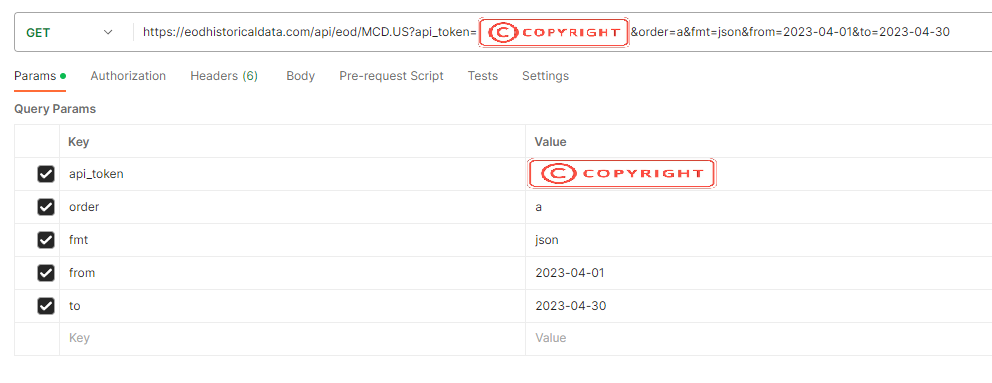
\includegraphics[scale=0.5]{images/postman.png}
\caption{Adatok lekérése Postman használatával (adatvédelmi okokból cenzúráztam a kulcsot)}
\label{fig:postman}
\end{figure}

\pagebreak

\subsection{Fejlesztői környezet }

A \textbf{Visual Studio Code} nyílt forráskódú kódszerkesztő, mely ingyenesen elérhető a fejlesztők számára. Az egyik legnépszerűbb alkalmazás, hiszen számos kiegészítővel rendelkezik, amely leveszi a terhet a felhasználó válláról, továbbá majdnem az összes ismert programozási nyelvet támogatja, például az általam is használt JavaScriptet, HTML-t, CSS-t és Node.js-t. 

A VS Code beépített támogatást tartalmaz az intelligens kódkezelésre az IntelliSense segítségével, mely nem csak a kód kiegészítésében és refaktorálásában, de a navigációban is hasznos lehet, főleg egy összetettebb projekt kapcsán. Továbbá beépített támogatást tartalmaz Node.js hibakereséshez és JavaScript fejlesztéséhez. Ezeken felül lehetőségünkben áll bővítményeket hozzáadni, mint például \emph{Live Server}, illetve rendelkezik beépített parancssorral, melyből így futtathattam a Node.js kódomat. \cite{vsc}

\subsubsection{Live Server}

A Visual Studio Code Elő Szerver (Live Server) bővítménye hihetetlenül hasznos a webfejlesztés folyamat során. Lehetővé teszi, hogy egy kattintással elindítsunk egy HTML dokumentumot és lefuttat egy dinamikusan generált szervert, amely során megnyit egy böngésző ablakot és feltölti az általunk kódolt elemekkel. A fájlon végrehajtott bármilyen gyakorlati módosítást követően a böngésző ablakát újratölti és azonnal végrehatja a változtatásokat. 

\subsection{Git }

A Git ingyenes, nyílt forráskódú verziókezelő rendszer, amelyet a kis és nagyon nagy projektek hatékony kezelésére használnak. A Git a forráskód változásainak nyomon követésére szolgál, lehetővé téve több fejlesztő számára, hogy együtt dolgozzon a fejlesztésen. Lényeges funkciója a verziókezelésen felül a Git Fa Objektum (Tree Object), amely hierarchikus kapcsolatot hoz létre a különböző könyvtárak és fájlok között. Ezáltal a fejlesztési folyamatokat külön ágakon lehet végezni, így elkerülhető az esedleges hibás kódolás terjesztése többi fejlesztő számára. Néhány fontosabb információ a Git-tel kapcsolatban: 

\begin{itemize}
\item Az elosztott verzióvezérlő eszköz a forráskód-kezelésre szolgál
\item Lehetővé teszi több fejlesztő együttműködését
\item Több ezer párhuzamos ágán keresztül támogatja a nemlineáris fejlesztést
\item Nyomon követi az előzményeket, illetve biztonsági mentéseket készít \cite{git}
\end{itemize}

Az általam készített alkalmazást regisztráltam a GitHub felhő alapú szolgáltatásán, amely tárolja a szükséges kódokat és fájlokat. Fejlesztésem során több ágon (branch) dolgoztam, így a forráskód, csakis abban az esetben került fel a fő (main) ágamra, ha a mellékágakon tesztelési folyamatok után sem találtam hibát.

\section{Kliens}

Először a Kezdőlap és Grafikonrajzoló oldalak funkcióival kezdtem az implementációt. Az \emph{index.html} fájlban létrehoztam a navigációhoz tartozó paneleket, majd CSS felhasználásával megalkottam a kinézetét és azt a kritikus funkciót, hogy a navigáció mindig a képernyő tetején legyen és kövesse annak a mozgását, így a felhasználó könnyedén tud lapozni az oldalak között. Mivel az oldalamat több felbontásra terveztem a reszponzivitás szemléletében, következésképpen itt is kulcs szerepet tölt be. Mivel a betűk eléggé nagyok, ezáltal bizonyos felbontás mellett egymásra halmozódnának, ezt elkerülve, ha az képernyő mérete kisebb mint 1099 pikszel, akkor a navigáció összecsukódik egy kis gombbá és a soros megjelenítést felváltja az oszlopos megvalósítás \aref{fig:navbarfunc}.

\begin{figure}[h]
\centering
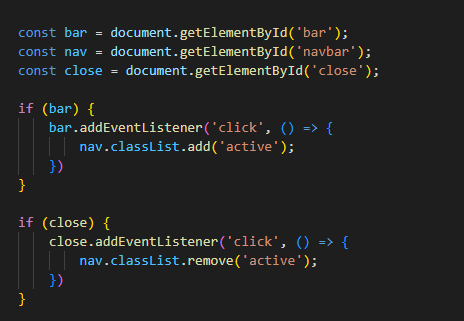
\includegraphics[scale=0.8]{images/navbarFunction.png}
\caption{A navigációs sáv összecsukása és kinyítása}
\label{fig:navbarfunc}
\end{figure}

További fejlesztés volt még az oldalak HTML vázának megvalósítása. Szükséges szempont volt, hogy a különböző oldalak más elemekkel töltsem fel, de alapjában véve egységes weboldal látszatát keltsék. A különböző részeket <section> címkével (tag) választom el, így átláthatóbb számomra, illetve néhány szekciót egyedi azonosítóval (id) láttam el, hogy működésüket, vagy külsejüket tudjam applikálni. A gombok és választható elemeknél a \textbf{Bootstrap} könyvtár beépített függvényeit használtam. A dátumokhoz tartozó gombokat jQuery függvény segítségével kiszelektálom és megjelenítek hozzájuk egy naptárat is. A naptáron lehetőség van kattintással kiválasztani az napot, vagy váltani a hónapo és évek között, illetve ha mégsem a megfelelő dátum lett kiválasztva, akkor törlés gomb megnyomásával hatálytalanítjuk a bevitt adatot \aref{fig:datepicker}.

\begin{figure}[h]
\centering
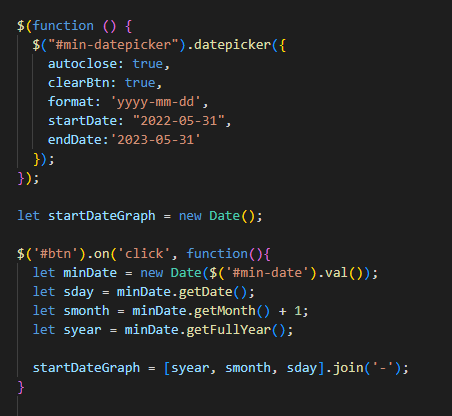
\includegraphics[scale=0.7]{images/datepicker.png}
\caption{A dátumválasztó működése kezdő dátumra}
\label{fig:datepicker}
\end{figure}

\pagebreak

A kliens egy API-n keresztül, HTTP kérésekkel kommunikál a szerverrel. A kommunikáció a úgy néz ki, hogy a \textbf{Grafikonrajzoló} oldalon található gomb megnyomásával inicializáljuk a rajzolót egy aszinkron függvény használatával. A függvény csak akkor hívódik meg, ha a felhasználó beállította a programhoz elengedhetetlen adattagokat, ilyen adattagok például a grafikon típusa, valamelyik befektetési alap és az árfolyamok közül az egyik kiválasztása, illetve a kezdeti és záró dátumok. Hogy ne kelljen minden egyes alkalommal minden adattagot újra beállítani, így alapértelmezetten kiválasztottam az első három opcióbol egyet.
	
	Az aszinkron függvény megvizsgálja, hogy a gomb felett található kettő dátum input fel van töltve adatokkal, tehát a felhasználó kiválaszotta a kezdő és a záró dátumot \aref{fig:validation}. 

\begin{figure}[h]
\centering
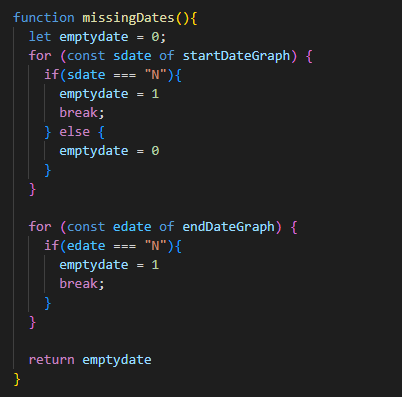
\includegraphics[scale=0.8]{images/dateValidation.png}
\caption{A missingDates fgv. megvizsgálja, hogy nincs-e üres dátum mező}
\label{fig:validation}
\end{figure}

Abban az esetben, ha üresek, akkor egy figyelmeztető üzenet jelenik meg, ami felhívja a figyelmet a dátumok kitöltésének feltételére. További feltételek még, hogy a kezdeti és záró dátum nem eshet ugyan arra a napra, illetve a záró dátum nem lehet kisebb mint a kezdeti dátum, hiszen az API hívásban problémát okozna a hibásan megadott időintervallum.

\begin{figure}[h]
\centering
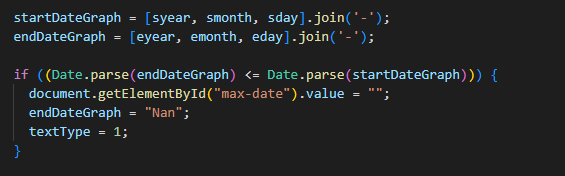
\includegraphics[scale=0.9]{images/emptyDate.png}
\caption{A kód felülvizsgálja a záró dátumot}
\end{figure}

Amennyiben minden mező sikeresen ki lett töltve a program GET kéréssel lekéri az adatokat a szerverről és átadja a weboldal címét, a felhasználó által kiválaszott tokent és a kezdeti, illetve a végső dátumokat. 

\begin{cpp}
const url = `http:/localhost:8080/api?ticker=${selectedInvest}&
             &start_date=${startDateGraph}&end_date=${endDateGraph}`;
\end{cpp} 

Ha sikerült a kérés és nem merült fel semmilyen hiba, akkor a függvény Promise-szal (ígéret) jelzi, hogy minden adat elérte a weboldalt \aref{fig:fetch}. Ezen adatokat a program json formátumban küldi fel, csakúgy mint ahogy backenden tárolva vannak, azzal a különbséggel, hogy csak azok az adattagok jöttek fel, amit a felhasználó kíválasztott.

\begin{figure}[h]
\centering
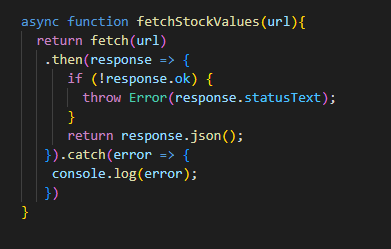
\includegraphics[scale=0.8]{images/fetch.png}
\caption{Backendről felküldött adatokat adja át a frontendnek json formátumban}
\label{fig:fetch}
\end{figure}

Most, hogy minden kért adat sikeresen elérte a klienst, következhet a diagram struktúrájának összetétele. Elsőként egy függvény felel azért, hogy megtudjuk milyen típusú adatok lettek kiválasztva. Ez a függvény mindig meghívódik gombnyomás előtt, hogy inicializálja a gárfot, ha esetleg az alapértelmezett opciók helyett más lehetőséget választott volna a felhasználó, majd utána gombnyomásra aktiválódik a folyamat újra.

\begin{figure}[h]
\centering
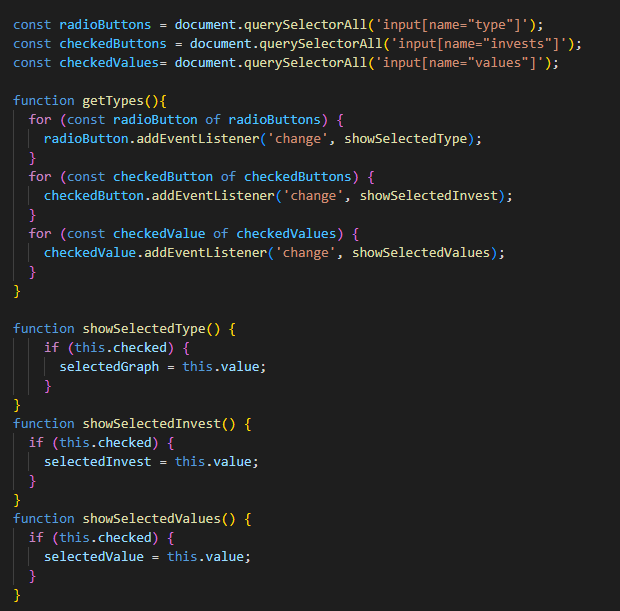
\includegraphics[scale=0.5]{images/types.png}
\caption{A getTypes fgv. a diagram típusainak változását figyeli}
\label{fig:fetch}
\end{figure}

A grafikon megvalósításához a Chart.js definiált könyvtárát használom fel. Ehhez HTML oldalon szükséges <canvas> címkét létrehozni, hiszen két dimenziós ábrát szeretnék megvalósítani. Egyedi azonosítóval láttam el a canvas elemet, amire a \emph{script.js} fájlban hivatkozok. A grafikonnak három fontos paraméterrel rendelkezik, úgy mint a típusa (types), adathalmaza (data) és opciói (options).

	A típúsát "switch" választási mechanizmussal érem el aképpen, hogy a felhasználó melyik befektetést választotta ki az oldalon, úgy az ahhoz tartozó megnevezést adom át a grafikonnak. 
Az adathalmazt egy függvény segítségével töltöm fel. Az API hívás során megkapott json fájlon végigiterál a függvény és egy tömbben adja vissza az adatokat amivel a grafikon tud dolgozni \aref{fig:chartData}. Az opcióit pedig json formátumban használom. A grafikon felett megjelenített idősávot függvény során valósítom meg, ami mindig a felhasználó által kiválasztott aktuális dátumot jeleníti meg, feltéve ha a dátumok megfelelnek a hibaellenőrzésnek. Animációval teszem látványosabbá a diagrammok megjelenítését.

\begin{figure}[h]
\centering
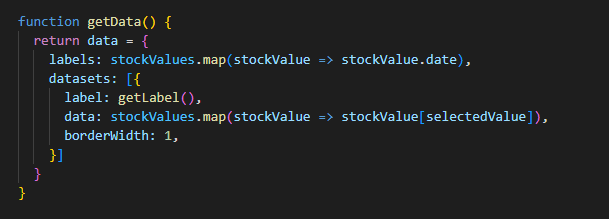
\includegraphics[scale=0.7]{images/chartData.png}
\caption{Az API hívás során megkapott adathalmazon iterál végig a getData fgv.}
\label{fig:chartData}
\end{figure}

Az alkalmazás felépítése úgy működik, hogy minden alkalommal amikor a "Mehet" gombot megnyomja a felhasználó az addig használt gráf úgymond megsemmisül és helyette a program új gráfot készít a megadott paraméterekkel \aref{fig:newChart}. Természetesen a feltételvizsgálat itt is fontos szerepet játszik, tehát ha nincs megadva dátum, akkor a hiba üzenet fog megjeleni és a gráf törlődik.

\begin{figure}[h]
\centering
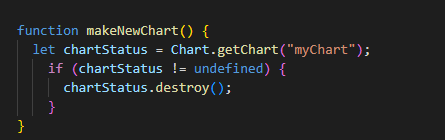
\includegraphics[scale=0.8]{images/makeNew.png}
\caption{A függvény megvizsgálja, hogy létezik gráf, ha igen, akkor törli azt}
\label{fig:newChart}
\end{figure}

\section{Szerver \label{fig:server}}

Ahhoz, hogy a szoftver működjön telepítenünk kell a megfelelő technológiákat és az architektúrát. Ahogy már a \textbf{Bevezetőben} ismertettem, a kliens-szerver architektúra megfelelő az alkalmazásra. A kliens egy böngészőben futtatott frontend, ami API hívásokon keresztül tud kommunikálni a backend szerverrel.
Hogy az architektúra működjön a számítógépünkön először telepíteni kell a Node.JS-t, és az Expresst. A Node.js-t egyszerűen le lehet tölteni a hivatalos honlapról \cite{nodeJS}. Windows-os felhasználóként az ehhez az operációs rendszerhez készített 64-bites setup segítségével telepítettem fel az alkalmazást. Hogy megbizonyosodjunk a \emph{node} sikeres letöltésről (lásd:\aref{fig:node}) bemutatok egy próba tesztet.

\begin{figure}[h]
\centering
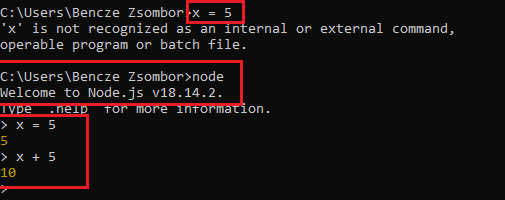
\includegraphics[scale=0.9]{images/nodeTest.png}
\caption{Sikeresen telepített node demó}
\label{fig:node}
\end{figure}

Miután megbizonyosodtunk, hogy sikeresen telepítettük a Node.js aktuális verzióját, használjuk a Visual Studio Code, vagy a Windows beépített terminálját és írjuk be a következő parancsot:
\begin{cpp}
npm init
\end{cpp} 
A kód lefutása után lehetőségünkben áll csomag nevet (package name), verziót (version), leírást (description), belépési pontot (entry point), teszt parancsot (test command), git adattárat (git repository), kulcsszavakat (keywords), szerzőt (author) és licenszt (license) megadni, de én azt javaslom az enter megnyomásával mindent hagyjunk meg a rendszernek, hogy automatikusan töltse ki helyettünk. Ha mindent jól csináltunk akkor létre kellett jönnie egy \emph{package.json} fájlnak. \aref{fig:package} A telepítésünk következő lépése a az \emph{Express.js} installálása, amit szintén a terminálon keresztül tudunk letölteni az alábbi paranccsal:
\begin{cpp}
npm install express --save
\end{cpp}

\begin{figure}[h]
\centering
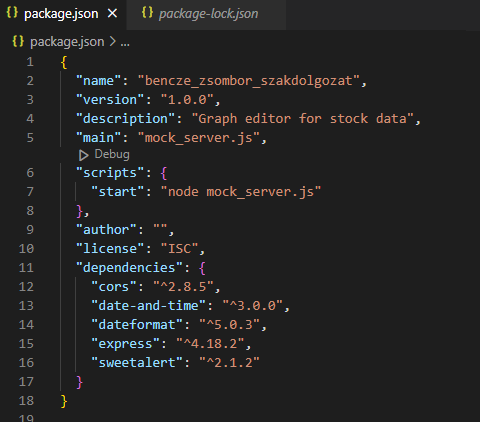
\includegraphics[scale=0.9]{images/packageJSON.png}
\caption{Az alkalmazáshoz készített package.json }
\label{fig:package}
\end{figure}

Észrevehetjük, hogy egy új mappa \emph{node\_modules} ékelődött be a fájlaink közé. Ez egy könyvtár, amelyet az npm hozott létre, és egy módja annak, hogy nyomon kövesse a helyileg telepített csomagokat. A felhasznált csomagok nevei és verziószámai, mind a \emph{package.json} nevű fájlban találhatók így, ha a GitHubra akarom menteni a projekteket, akkor időt sprólok, hiszen nem nekem kell egyesével több ezer fájlt feltöltenem a felhőbe, mert mindegyik megtalálható lesz a json-ben. Az ábrán \aref{fig:package} látható dependenciák (dependencies) tartalmazza mindazokat a telepítéseket amiket az alkalmazáshoz használtam.

	A telepítést követően létre kell hoznunk a webszervert portját, amit az Express csomag segítségével létrehoztam. A szerver alapját úgy állítottam be, hogy a 8080-as porton figyeljen, azaz a böngészőben a http://localhost:8080 címen legyen elérhető.

\begin{figure}[h]
\centering
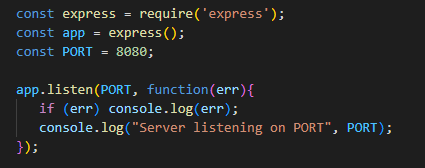
\includegraphics[scale=1]{images/serverPort.png}
\caption{Ezen a porton lehet elérni a szervert}
\end{figure}

A szerver működtetéséhez már csak egy lépés van hátra, mégpedig létrehozni magát a tényleges http szervert. A kódot úgy írtam meg, hogyha a szerver 200-as státuszkódot kap, tehát nem történt hiba a szerver elérésében, akkor a "req" argumentet felhasználva a kód lekéri a klienstől az URL-t, továbbá meghív egy "getData" nevű függvényt, amit később fogok ismertetni. \cite{nodeServer}

\begin{figure}[h]
\centering
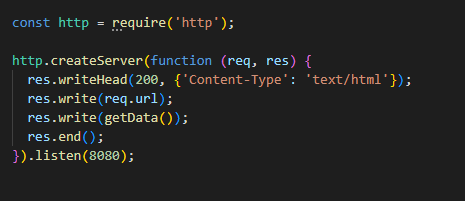
\includegraphics[scale=1]{images/createServer.png}
\caption{Szerver létrehozása}
\end{figure}


A szerver REST API-n keresztül hallgat a kérésekre. Ezen az API-n szolgálja fel a statikus tőzsdei adatokat, amiket backend/data mappába mentettem el és Postman  (lásd: \aref{fig:postman}) segítségével "GET" kéréssel értem el az adatokat. Mivel az alkalmazás hat különböző befektetést ismertet, így hat API hívást intéztem, amelyeket json fájlban tároltam, hogy könnyen feltudjam küldeni őket a kliensre.

\begin{figure}[h]
\centering
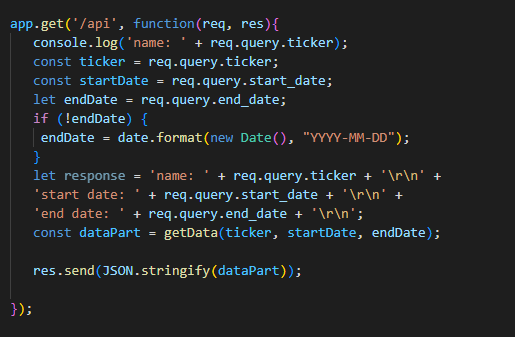
\includegraphics[scale=0.8]{images/apiCall.png}
\caption{Az alábbi képen láthatóak a metódusok, amin keresztül meghívódnak az árfolyam adatok}
\end{figure}

Mivel a szerver és a kliens nem egy URL címen futnak, ezért globálisan össze kell őket hangolni, amihez szükség van egy keresztező erőforrás megosztásra (Cross-Origin Resource Sharing) röviden: CORS. 
 
\pagebreak

\begin{cpp}
let cors = require('cors')

app.use(cors({
   origin: '*'
}));
\end{cpp} 

Most, hogy a szerver és a kliens is sikeresen kommunikál egymással, már csak lépés van hátra, mégpedig a felhasználó által igényelt adatok elérése. A weboldalon felhasználónak lehetősége adódik kiválasztani, hogy melyik befektetést szeretné megjeleníteni, illetve kitud választani két dátumot, miszerint mettől (kezdeti dátum input) meddig (záró dátum input) szeretné megjeleníteni a grafikonrajzolóval a kívánt gráfot. Majd ezeket a dátumot adatokat a kliens leküldi a szervernek, amely megkapva feldolgozza és a kért paraméterek alapján megszűri az adott json-t és úgy küldi vissza a kliensnek.

\begin{figure}[h]
\centering
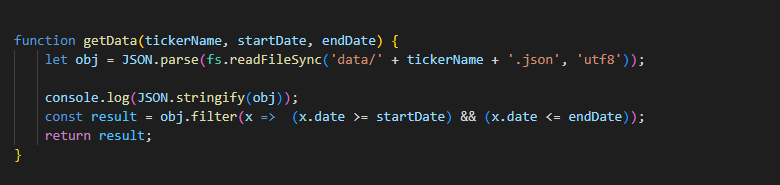
\includegraphics[scale=0.7]{images/getData.png}
\caption{Frontend-ről megkapott adatok alapján kiválasztja a kezdeti és záró dátumon belüli értékeket}
\end{figure}
\Chapter{Tesztelés}

A fejezetben be kell mutatni, hogy az elkészült alkalmazás hogyan használható.
(Az, hogy hogyan kell, hogy működjön, és hogy hogy lett elkészítve, az előző fejezetekben már megtörtént.)

Jellemzően az alábbi dolgok kerülhetnek ide.
\begin{itemize}
\item Tesztfuttatások. Le lehet írni a futási időket, memória és tárigényt.
\item Felhasználói kézikönyv jellegű leírás. Kifejezetten a végfelhasználó szempontjából lehet azt bemutatni, hogy mit hogy lehet majd használni.
\item Kutatás kapcsán ide főként táblázatok, görbék és egyéb részletes összesítések kerülhetnek.
\end{itemize}

\Chapter{Összefoglalás}

A szakdolgozatom pénzügyi adatok elemzéséhez használható interaktív megjelenítő weboldalt mutatott be elméleti és gyakorlati példákkal egyetemben, valamint a hozzá elkészített alkalmazást. A dolgozat felépítése jellemzően az elméleti tudástárból a gyakorlati megvalósítás felé terjedt. Az elméleti részben feltártam a Grafikonrajzoló lapon elérhető diagrammok típusait, ismertettem tőzsdei alapfogalmakat, illetve kifejtettem az oldalon található kulcsszavakat, amelyek tudása elengedhetetlen. Ezek után az általam írt program tervezésének lépéseit mutattam be, majd a hozzá felhasznált technológiákat részleteztem.

	Az alkalmazás fejlesztése Visual Studio Code környezetben történt, munkámat elősegítette a Live Server bővítmény által kínált kényelmes élő szerver szolgáltatás. A szerverhez használt kódokat Node.js nyelven írtam meg és az adatokat az EOD Historical Data nevezetű webhely szolgáltatta. Mivel az portálon fellelhető teljes adatkészlet nem elérhető ingyenes verzióban, ezért ezt a problémát úgy abszolváltam, hogy Postman alkalmazás segítségével lekértem a hat befeketetésem adatait és külön json fájlban mentettem el őket. Az alkalamzás ezen adatok 1 éves halmazával tud operálni. 

	A klienst JavaScript és jQuery nyelveken vittem véghez, emellett HTML elemekkel építettem fel a sémáját, továbbá CSS és Bootstrap komponensekkel vittem véghez a megjelenésének kialakítását. A gráfok szerkezetében a Chart.js előre definiált könyvtárát vettem igénybe és úgy alakítottam, hogy prominens legyen a látogató számára. Úgy gondoltam, hogy ne kelljen mindig végigkattintani a diagrammok adatait, ezáltal a Grafikonrajzoló három opciójának alapértelmezett választásként adtam meg, amiket természetesen lehet kombinálni a felhasználó igénye szerint. A grafikon megjelenésének nélkülözhetetlen részei a kezdeti és záró dátumok, ennek okán csakis akkor jelenik meg ha a vizsgálati feltételeknek eleget tévő paraméterek kerülnek kijelölésre. Ehhez szükséges a szerver és kliens kommunikációja amit API hívásokon keresztül valósítottam meg.

	A kész szoftver legnagyobb előnye, hogy önálló weboldalként is képes megállni a helyét. Struktárja modern webfejlesztési módszerek szerint készült, tehát könnyen kezelhető, gyorsan működik és interaktív.A program a grafikonok változatos megjelenítésével, emellett többféle árfolyam lehetőségével szándékozik kiemelkedni a többi hasonló pénzügyi adatokat elemző alkalmazások közül. 

	Véleményem szerint sikerült egy működő weboldalt létrehoznom, amihez néhány továbbfejlesztési lehetőség ötletével álltam elő.

\section{Továbbfejlesztési lehetőségek}

A szakdolgozatom készítése alatt rengeteg ötlet és koncepció jutott eszembe, de mivel a rendelkezésre álló idő végleges, így korlátoznom kellett magam a fontosabb funkciók megalkotására. Az első és talán legszembetűnőbb opció ami nincs a szoftveremnél az adatbázis. A Tervezési fázisnál még szerepelt, de később elvetettem az ötletet, mert nem éreztem feltétlenül szükségesnek. Döntésemet az is indokolta, mint ahogy a dolgozatom címében is szerepel "Interaktív megjelenítő eszköz", így az energiaforrást a grafikonrajzolóra fordítottam. Viszont ha mondjuk a tanulmányaim során megismert MySQL adatbázist bevezettem volna, akkor az ötödik fejezetben említett hiányzó funkciók közül kettőt kipipálhatok.

	Amivel még lehet emelni az oldal színvonlát, ha több befektetés áll rendelkezésre, és egyszerre nem csak egy alapot lehet kiválasztani. Ezen funkció nagyon átgondolt struktúrát igényel, mert ha több alapot is ki lehet választani, akkor mindegyik megjelenítési típusnál le kell tesztelni miként működik. Hiszen ami mondjuk működőképes egy vonaldiagramnál, az nem biztos, hogy hasonlóképpen működne a kördiagramnál. Tehát alaposan kell tanulmányozni a diagrammok típusait, hogy milyen szabályosságok érvényesek a különféle típusokra és a kellő háttérinformáció megszerzése után úgy kellene megtervezni a rendszert, hogy minden elemre működjön. Talán ezért is hiányzik a rangosabb oldalakról a többféle típus kiválasztása.

	Amit még a kutatásaim során néhány oldalon felfedeztem, az a bejelentkezés és profil részleg kialakítása. A szubjektív véleményem, hogy nem tartom túl szükséges elemnek egy ilyesfajta weboldalon, de példának okáért egy alternatívaként arra hasznos lehet, hogy a kedvenc részvényeket nyomon lehessen követni.

\section{Summary}

My thesis presented an interactive display website that can be used for analyzing financial data, together with theoretical and practical examples, as well as the application prepared for it. 
The structure of the thesis typically extended from the theoretical knowledge base to the practical implementation. 
In the theoretical part, I explored the types of diagrams available on the Graph Drawing tab, explained basic stock concepts, and explained the keywords on the page, of which knowledge is essential. After that, I presented the steps of designing the program that I wrote, and then detailed the technologies used for it.

	The application was developed in the Visual Studio Code environment, my work was facilitated by the convenient live server service offered by the Live Server extension. The code that used for the server is written by Node.js and the data was provided by the EOD Historical Data website. 
Since the complete data set found on the portal is not available in the free version, I solved this problem by using the Postman application to retrieve the data of my six blackouts and save them in a separate json file. The application can operate with a 1-year set of these data.

	I implemented the client in JavaScript and jQuery languages, in addition, I built its schema with HTML elements, and I implemented the design of its appearance with CSS and Bootstrap components. In the structure of the graphs, I used the predefined library of Chart.js and designed it so that it is prominent for the visitor. I thought that it would not be necessary to always click through the data of the charts, so I gave a default choice for the three options of the Graphic Designer, which of course can be combined according to the user's needs. The start and end dates are indispensable parts of the appearance of the graph, which is why they only appear when parameters that meet the test conditions are selected. This requires server and client communication, which I implemented through API calls.

	The biggest advantage of the ready-made software is that it can also stand its ground as an independent website. Its structure is made according to modern web development methods, so it is easy to use, works quickly and is interactive. The program intends to stand out from other applications that analyze similar financial data with the varied display of graphs and, in addition, the possibility of multiple exchange rates.


\clearpage

\addcontentsline{toc}{chapter}{Irodalomjegyzék}
\bibliographystyle{plain}
\bibliography{dolgozat.bib}

\newpage

\pagestyle{empty}

\noindent \textbf{\Large CD Használati útmutató}

\vskip 1cm

\textit{A mellékelt CD tartalma}
\begin{itemize}
\item frontend mappa: tartalmazza a program kliens oldali forráskódját.
\item backend mappa: tartalmazza a program szerver oldali forráskódját.
\item szakdolgozat mappa: tartalmazza a szakdolgozat \LaTeX{} forráskódját
\item Szakdolgozat.pdf: tartalmazza a szakdolgozat PDF formátumban
\item GitHub link: tartalmazza az elkészített program \textbf{GitHub} linkjét.
\end{itemize}

\vskip 1cm

\textit{A program futtatása}

A programok használatához, szükséges a negyedik fejezetben említett függőségek telepítése. 

\begin{itemize}
\item Töltsük le a Visual Studio Code-t a böngészőről és adjuk hozzá a live server bővítményt.
\item Töltsük le a Node.js-t a hivatalos oldalról. (link: https://nodejs.org/en\#home-downloadhead)
\item Lépjünk be a backend mappába és írjuk be az alábbi parancsokat a terminálba:
\begin{cpp}
 npm install
 npm run start
\end{cpp}
\item Ha a terminál azt az üzenetet írta ki, hogy: "Server listening on PORT 8080", akkor már csak a Live Server van hátra
\item Jobb kattintás a frontend/index.html fájlra és "Open with Live Server"
\end{itemize}


\end{document}
